\chapter{Significado de la derivada}

    \begin{def.}
	Sea $f$ una función y $A$ un conjunto de números contenido en el dominio de $f$. Un punto $x$ de $A$ es un punto máximo de $f$ en $A$ si
	$$f(x)\geq f(y)\qquad \mbox{para todo} \; y \; \mbox{de}\; A.$$
	El número $f(x)$ se denomina el \textbf{valor máximo} de $f$ en $A$ (y también diremos que $f$ alcanza su valor máximo en el punto $x$ de $A$).\\\\
	$f$ tiene un \textbf{mínimo} en el punto $x$ de $A$ si $-f$ tiene un máximo en el punto $x$ de $A$.
    \end{def.}

En general, nos interesará el caso en que $A$ es un intervalo cerrado $[a,b];$ si $f$ es continua, entonces el Teorema 7-3 garantiza que $f$ alcanza realmente dicho valor máximo en $[a,b].$\\

Ahora ya estamos en condiciones para enunciar un teorema que ni siquiera depende de la existencia de cotas superiores mínimas.\\

\begin{teo}
    Sea $f$ cualquier función definida en $(a,b)$. Si $x$ es un punto máximo (o mínimo) de $f$ en $(a,b)$ y $f$ es diferenciable en $x$, entonces $f'(x)=0.$ (Observemos que no hemos supuesto la diferenciabilidad, ni siquiera la continuidad, de $f$ en otros puntos.)\\\\
	Demostración.-\; Consideremos el caso en que $f$ tiene un máximo en $x$. Si $h$ es cualquier número tal que $x+h$ pertenece a $(a,b)$, entonces
	$$f(x)\geq f(x+h),$$
	ya que $f$ tiene un máximo en el punto $x$ de $(a,b)$. Esto significa que 
	$$f(x+h)-f(x)\leq 0.$$
	De manera que, si $h>0$ tenemos
	$$\dfrac{f(x+h)-f(x)}{h}\leq 0,$$
	y por tanto
	$$\lim_{h\to 0^+}\dfrac{f(x+h)-f(x)}{h}\leq 0.$$
	Por otra parte, si $h<0$, tenemos
	$$\dfrac{f(x+h)-f(x)}{h}\geq 0,$$
	o sea
	$$\lim_{h\to 0^-}\dfrac{f(x+h)-f(x)}{h}\geq 0.$$
	Por hipótesis, $f$ es diferenciable en $x$, de manera que ambos límites deben ser iguales (de hecho son iguales a $f'(x)$). Esto significa que
	$$f'(x)\leq 0\quad \mbox{y}\quad f'(x)\geq 0,$$
	de lo cual se deduce que $f'(x)=0.$\\
\end{teo}

    \begin{def.}
	Sea $f$ una función, y $A$ un conjunto de números contenido en el dominio de $f$. Un punto $x$ de $A$ es un \textbf{punto máximo [mínimo] local} de $f$ en $A$ si existe algún $\delta>0$ tal que $x$ es un punto máximo [mínimo] de $f$ en $A\cap (x-\delta,x+\delta.)$
    \end{def.}

\begin{teo}
    Si $x$ es un máximo o mínimo local de $f$ en $(a,b)$ y $f$ es diferenciable en $x$, entonces $f'(x)=0$.\\\\
	Demostración.-\; Se trata de una aplicación del teorema 1 (capítulo 11, Spivak).
\end{teo}

El recíproco del teorema 2 no es cierto; la condición $f'(0)$ no implica que $x$ sea un punto máximo o mínimo local en $f$. Precisamente por esta razón, se ha adoptado una terminología especial para describir a aquellos números $x$ que satisfacen la condición $f'(0)$.

    \begin{def.}
	Un \textbf{punto critico} de una función $f$ es un número $x$ tal que 
	$$f'(x)=0.$$
	Al número $f(x)$ se le denomina \textbf{valor critico} de $f$.
    \end{def.}

Consideremos en primer lugar el problema de hallar el máximo o el mínimo de $f$ en un intervalo cerrado $[a,b]$. (En este caso, si $f$ es continua, sabemos que dicho valor máximo y mínimo debe existir.) Para localizarlos, deben considerarse tres clases de puntos:

\begin{enumerate}[(1)]
    \item Los puntos críticos de $f$ en $[a,b]$.
    \item Los puntos extremos $a$ y $b$.
    \item Aquellos puntos $x$ de $[a,b]$ tales que $f$ no es diferenciable en $x$.
\end{enumerate}

Si $x$ no pertenece al segundo no al tercer grupo entonces forzosamente debe pertenecer al primero.\\


\begin{obs}
    En el capítulo 7 ya resolvimos el problema de este tipo cuando demostramos que si $n$ es par, la función
    $$f(x)=x^n+a_{n-1}x^{n-1}+\ldots + a_0$$
    tiene un valor mínimo en toda la recta real. Dicho valor mínimo se puede encontrar resolviendo la ecuación, si es posible, y comparando los valores de $f(x)$ en dichos $x$.\\
\end{obs}

\begin{teo}[Teorema de Rolle]
    Si $f$ es continua en $[a,b]$ y diferenciable en $(a,b)$, y $f(a)=f(b)$, entonces existe un número $x$ en $(a,b)$ tal que $f'(x)=0$.\\\\
	Demostración.-\; A partir de la continuidad en $f$ en $[a,b]$ deducimos que $f$ tiene valor máximo y mínimo en $[a,b]$. Supongamos primero que el valor máximo se presenta en un punto $x$ de $(a,b)$. Entonces $f'(x)=0$ según el teorema 1, y la demostración queda completa. Supongamos ahora que el valor mínimo de $f$ se presenta en algún punto $x$ de $(a,b)$. Entonces, de nuevo $f'(x)=0$ según el teorema 1. Finalmente, supongamos que los valores máximo y mínimo se presentan ambos en los extremos del intervalo. Como $f(a)=f(b),$ dichos valores coinciden, de manera que $f$ es una función constante, y en este caso se puede elegir cualquier valor $x$ de $(a,b)$.
\end{teo}

\begin{teo}[Teorema del valor medio] \hypertarget{def1}
    Si $f$ es continua en $[a,b]$ y diferenciable en $(a,b)$, existe un número $x$ en $(a,b)$ tal que 
    $$f'(x)=\dfrac{f(b)-f(a)}{b-a}.$$\\
	Demostración.-\; Sea 
	$$h(x)=f(x)-\left[\dfrac{f(b)-f(a)}{b-a}\right](x-a).$$
	Evidentemente, $h$ es continua en $[a,b]$ y diferenciable en $(a,b)$, y 
	$$h(a)=f(a),\qquad h(b)=f(b)-\left[\dfrac{f(b)-f(a)}{b-a}\right](b-a)=f(a).$$
	Por tanto, se puede aplicar el teorema de Rolle a la función $h$ y deducir que existe algún $x$ en $(a,b)$ tal que
	$$0=h'(x)=f'(x)-\dfrac{f(b)-f(a)}{b-a},$$
	de modo que 
	$$f'(x)=\dfrac{f(b)-f(a)}{b-a}.$$\\
\end{teo}

\begin{cor}
    Si $f$ está definida en un intervalo y $f'(x)=0$ en todo $x$ del intervalo, entonces $f$ es constante en dicho intervalo.\\\\
	Demostración.-\; Sean $a$ y $b$ dos puntos del intervalo con $a\neq b$. Entonces existe algún $x$ de $(a,b)$ tal que 
	$$f'(x)=\dfrac{f(b)-f(a)}{b-a}.$$
	Pero $f'(x)=0$ para todo $x$ del intervalo, por tanto
	$$0=\dfrac{f(b)-f(a)}{b-a},$$
	y por consiguiente $f(a)=f(b)$. Así pues, el valor de $f$ en dos puntos cualesquiera del intervalo es el mismo, lo cual significa que $f$ es constante en el intervalo.\\\\
\end{cor}

\begin{cor}
    Si $f$ y $g$ están definidas en el mismo intervalo y $f'(x)=g'(x)$ para todo $x$ del intervalo, entonces existe algún número $c$ tal que $f=g+c.$\\\\
	Demostración.-\; Para todo $x$ del intervalo se verifica que $(f-g)'(x)=f'(x)-g'(x)=0,$ de manera que, según el corolario 1, existe un número $c$ tal que $f-g=c.$
\end{cor}

    \begin{def.}
	Una función es \textbf{creciente} en un intervalo si $f(a)<f(b)$ siendo $a$ y $b$ dos números del intervalo con $a<b$. La función $f$ es \textbf{decreciente} en un intervalo si $f(a)>f(b)$ para todo $a$ y $b$ del intervalo con $a<b$. (A menudo se dice simplemente que $f$ es creciente o decreciente, en cuyo caso se deduce que el intervalo es el dominio de $f$.) 
    \end{def.}

\begin{cor}
    Si $f'(x)>0$ para todo $x$ de un intervalo, entonces $f$ es creciente en dicho intervalo; si $f'(x)<0$ para todo $x$ del intervalo, entonces $f$ es decreciente en dicho intervalo.\\\\
	Demostración.-\; Consideremos el caso en que $f'(x)>0$. Sean $a$ y $b$ dos puntos del intervalo con $a<b$. Entonces existe algún punto $x$ en $(a,b)$ que verifica
	$$f'(x)=\dfrac{f(b)-f(a)}{b-a}.$$
	Pero $f'(x)>0$ para todo $x$ en $(a,b)$, por tanto 
	$$\dfrac{f(b)-f(a)}{b-a}>0.$$
	Como $b-a>0$ se deduce que $f(b)>f(a).$\\\\
	Consideremos ahora el caso en que $f'(x)<0$. Sean $a$ y $b$ dos puntos del intervalo con $a<b$. Entonces existe algún punto $x$ en $(a,b)$ que verifica
	$$f'(x)=\dfrac{f(b)-f(a)}{b-a}.$$
	Pero $f'(x)<0$ para todo $x$ en $(a,b)$, por tanto 
	$$\dfrac{f(b)-f(a)}{b-a}<0.$$
	De donde se deduce que $f(b)<f(a).$\\
\end{cor}

Podemos dar un esquema general para decidir si un punto crítico es un máximo local, un mínimo local o ninguna de las dos cosas:

\begin{enumerate}[(1)]
    \item Si $f'>0$ en algún intervalo a la izquierda de $x$ y $f'<0$ en algún intervalo a la derecha de $x$, entonces $x$ es un punto máximo local.
    \item  Si $f'<0$ en algún intervalo a la izquierda de $x$ y $f'>0$ en algún intervalo a la derecha de $x$, entonces $x$ es un punto mínimo local.
    \item Si $f'$ tiene el mismo signo en algún intervalo a la izquierda de $x$ que en algún intervalo a la derecha, entonces $x$ no es ningún punto máximo ni mínimo local.
\end{enumerate}

En varios problemas de este capítulo y de capítulos sucesivos se pide hacer una representación gráfica de funciones. En cada caso debe determinar

\begin{enumerate}[(1)]
    \item los puntos críticos de $f$,
    \item el valor de $f$ en los puntos críticos,
    \item el signo de $f'$ en las regiones entre los puntos críticos (si esto no está claro ya),
    \item los números $x$ tales que $f(x)=0$ (si es posible),
    \item el comportamiento de $f(x)$ cuando $x$ se hace grande o grande negativo (si es posible).
\end{enumerate}

Existe un criterio popular para hallar los máximos y mínimos locales, que depende del comportamiento de la función sólo en los puntos críticos.\\

%------------------- teorema 5 ----------------------------
\begin{teo}
    Supongamos que $f'(a)=0.$ Si $f''(a)>0,$ entonces $f$ tiene un mínimo local en $a$; si $f''(a)<0,$ entonces $f$ tiene un máximo local en $a.$\\\\
	Demostración.-\; Por definición,
	$$f''(a)=\lim_{h\to 0}\dfrac{f'(a+h)-f'(a)}{h}.$$
	Como $f'(a)=0$, esta igualdad puede escribirse como
	$$f''(a)=\lim_{h\to 0}\dfrac{f'(a+h)}{h}.$$
	Supongamos ahora que $f''(a)>0$. Entonces $\dfrac{f'(a+h)}{h}$ ha de ser positivo para valores suficientemente pequeños de $h$. Por tanto:
	\begin{center}
	    $f'(a+h)$ ha de ser positivo para valores de $h>0$ suficientemente pequeños. Y
	    $f'(a+h)$ ha de ser negativo para valores de $h<0$ suficientemente pequeños.
	\end{center}
	Esto significa por el corolario 3 (Spivak, capitulo 11) que $f$ es creciente en algún intervalo a la derecha de $a$ y $f$ es decreciente en algún intervalo a la izquierda de $a$. Por consiguiente, $f$ tiene un mínimo local en $a$. La demostración es análoga en el caso de que $f''(a)<0.$\\
\end{teo}

Aunque el Teorema 5 es muy útil en el caso de funciones polinómicas, para muchas otras funciones la segunda derivada es tan complicada que es más fácil considerar el signo de la primera derivada. Además, si a es un punto crítico de $f$ puede ocurrir que $f''(a)=0$. En este caso, el Teorema 5 no proporciona información: es posible que a sea un punto máximo local, un mínimo local o ninguna de las dos cosas.\\

%-------------------- teorema 6 -----------------------------
\begin{teo}
    Supongamos que $f''(a)$ existe. Si $f$ tiene mínimo local en $a$, entonces $f''(a)\geq 0$; si $f$ tiene un máximo local en $a$, entonces $f''(a)\leq 0.$\\\\
	Demostración.-\; Supongamos que $f$ tiene un mínimo local en $a$. Si $f''(a)<0$, entonces $f$ tendría también un máximo local en $a$, por el teorema $5$. Es decir, $f$ sería constante en algún intervalo que contiene a $a$, y por tanto $f''(a)=0$, lo cual es una contradicción. Por tanto, debe verificarse que $f''(a)\geq 0$. El caso de un máximo loca se trata de manera análoga.\\
\end{teo}

%-------------------- teorema 7. -----------------------------
\begin{teo}
    Supongamos que $f$ es continua en $a$ y que $f'(x)$ existe para todo $x$ de algún intervalo que contiene a $a$, excepto quizás en $x=a$. Supongamos, además, que $\lim\limits_{x\to 0}f'(x)$ existe. Entonces $f'(a)$ también existe y 
    $$f'(a)=\lim\limits_{x\to a}f'(x).$$\\
	Demostración.-\; Por definición,
	$$f'(a)=\lim\limits_{h\to 0}\dfrac{f(a+h)+f(a)}{h}.$$
	Para valores de $h>0$ suficientemente pequeños, la función $f$ es continua en $[a,a+h]$ y diferenciables en $(a,a+h)$ (lo mismo ocurre para valores de $h<0$ suficientemente pequeños). Según el teorema del valor medio, existe un número $\alpha_h$ en $(a,a+h)$ tal que 
	$$\dfrac{f(a+h)-f(a)}{h}=f'(\alpha_h).$$
	Además $\alpha_h$ tiende a $a$ cuando $h$ tiende a $0$, ya que $\alpha_h$ pertenece al intervalo $(a,a+h)$; como $\lim\limits_{x\to a}f'(x)$ existe, se deduce que 
	$$f'(a)=\lim_{h\to 0}\dfrac{f(a+h)-f(a)}{h}=\lim_{h\to 0}f'(\alpha_h)=\lim_{x\to a}f'(x).$$
	En otras palabras, sean $L=\lim\limits_{x\to a}f'(x)$, por definición de límite se tiene 
	\begin{center}
	    Para todo $\epsilon>0$, existe un $\delta>0$ tal que, si $0<|x-a|<\delta$, entonces $|f'(x)-L|<\epsilon.$
	\end{center}
	Ahora, si $0<|x-a|<\delta$ podríamos utilizar el teorema del valor medio para encontrar un punto $c$ entre $a$ y $x$ que satisfaga,
	$$\dfrac{f(x)-f(a)}{x-a}=f'(c).$$
	Notemos que $c$ satisface también a $0<|c-a|<\delta,$ tal que $|f'(c)-L|<\epsilon.$ Como consecuencia 
	$$\left|\dfrac{f(x)-f(a)}{x-a}-L\right|<\epsilon.$$ 
	Es decir,
	$$0<|x-a|<\delta \quad \Rightarrow \quad \left|\dfrac{f(x)-f(a)}{x-a}-L\right|<\epsilon.$$
	Por lo tanto, $$f'(a)=L.$$\\
\end{teo}

Incluso si $f$ es una función diferenciable en todo punto, es posible que $f'$ sea discontinua. Por ejemplo
$$f(x)=\left\{\begin{array}{ll}
    x^2\sen\dfrac{1}{x},&x\neq 0\\\\
    0,&x=0\\
\end{array}\right.$$

Ahora veremos una generalización del teorema del valor medio.\\\\

%-------------------- teorema 8. -----------------------------
\begin{teo}[Torema del valor medio de Cauchy]
    Si $f$ y $g$ son continuas en $[a,b]$ y diferenciables en $(a,b)$, entonces existe un número $x$ en $(a,b)$ tal que 
    $$[f(b)-f(a)]g'(x)=[g(b)-g(a)]f'(x).$$
    (Si $g(b)\neq g(a)$ y $g'(x)\neq 0$, esta ecuación puede escribirse como
    $$\dfrac{f(b)-f(a)}{g(b)-g(a)}=\dfrac{f'(x)}{g'(x)}.$$
    Observemos que si $g(x)=x$ para todo $x$, entonces $g'(x)=1$, y se obtiene el teorema del valor medio. Por otra parte aplicando el Teorema del valor medio a $f$ y a $g$ por separado, se deduce que existen un $x$ e $y$ en $(a,b)$ que verifican
    $$\dfrac{f(b)-f(a)}{g(b)-g(a)}=\dfrac{f'(x)}{g'(y)};$$
    pero no existe ninguna garantía de que los $x$ e $y$ hallados de esta manera sean iguales.
    Estas consideraciones pueden hacer pensar que el Teorema del Valor Medio de Cauchy es muy difícil de demostrar, pero en realidad basta aplicar uno de los artilugios más simples.)\\\\
	Demostración.-\; Sea 
	$$h(x)=f(x)\left[g(b)-g(a)\right]-g(x)\left[f(b)-f(a)\right].$$
	Entonces $h$ es continua en $[a,b]$, diferenciable en $(a,b)$ y 
	$$h(a)=f(a)g(b)-g(a)f(b)=h(b).$$
	Según el teorema de Rolle, $h'(x)=0$ para algún $x$ de $(a,b)$, lo que significa que 
	$$0=f'(x)\left[g(b)-g(a)\right]-f'(x)\left[f(b)-f(a)\right].$$
\end{teo}

El Teorema del Valor Medio de Cauchy es la herramienta básica necesaria para demostrar un teorema que facilita el cálculo de límites de la forma
$$\lim_{x\to a}\dfrac{f(x)}{g(x)}.$$
cuando
$$\lim_{x\to a}f(x)=0\quad \mbox{y}\quad \lim_{x\to a}g(x)=0.$$
En este caso no es aplicable el Teorema 5.2.\\\\

%-------------------- teorema 9. -----------------------------
\begin{teo}[Regla de L'Hopital]
    Supongamos que 
    $$\lim_{x\to a}f(x)=0 \quad \mbox{y}\quad \lim_{x\to a}g(x)=0,$$
    y supongamos también que $\lim\limits_{x\to a}f'(x)/g'(x)$ existe. Entonces $\lim\limits_{x\to a}f(x)/g(x)$ existe y 
    $$\lim_{x\to a}\dfrac{f(x)}{g(x)}=\lim_{x\to a}\dfrac{f'(x)}{g'(x)}.$$
    (Observe que el teorema 7 es un caso particular.)\\\\
	Demostración.-\; La hipótesis de que el $\lim\limits_{x\to a}f'(x)/g'(x)$ existe contiene dos suposiciones implícitas:
	\begin{enumerate}[(1)]
	    \item existe un intervalo $(a-\delta,a+\delta)$ tal que $f'(x)$ y $g'(x)$ existen para todo $x$ de $(a-\delta,a+\delta)$ excepto quizás para $x=a$,
	    \item en este intervalo $g'(x)\neq 0$ excepto quizás, de nuevo, en $x=a.$
	\end{enumerate}
\end{teo}
Por otra parte, no se supone ni siquiera que $f$ y $g$ estén definidas en el punto $a$. Si definimos $f(a)=g(a)=0$ (cambiando, si es necesario, los valores previos de $f(a)$ y $g(a)$), entonces $f$ y $g$ son continuas en el punto $a$. Si $a<x<a+\delta$, puede aplicarse a $f$ y a $g$ el Teorema del Valor Medio y el Teorema del Valor Medio de Cauchy en el intervalo $[a,x]$ (y lo mismo ocurre en el caso de que $a-\delta < x < a$). Aplicando en primer lugar el Teorema del Valor Medio a $g$, vemos que $g(x)\neq 0$, ya que si $f(x)=0$ entonces existiría algún $x_1$ en $(a,x)$ tal que $g'(x_1)=0$, lo que contradice (2). Aplicando ahora el Teorema del Valor Medio de Cauchy a $f$ y a $g$, vemos que existe un número $\alpha_x$ en $(a,x)$ tal que 
$$\left[f(x)-0\right]g'(\alpha_x)=\left[g(x)-0\right]f'(\alpha_x)$$
o
$$\dfrac{f(x)}{g(x)}=\dfrac{f'(\alpha_x)}{g'(\alpha_x)}.$$
Pero $\alpha_x$ se aproxima a $a$ cuando $x$ se aproxima a $a$, ya que $\alpha_x$ está en el intervalo $(a,x)$; como estamos suponiendo que $\lim\limits_{y\to a}f'(y)/g'(y)$ existe, se deduce que
$$\lim_{x\to a}\dfrac{f(x)}{g(x)}=\lim_{x\to a}\dfrac{f'(\alpha_x)}{g'(\alpha_x)}=\lim_{y\to a}\dfrac{f'(y)}{g'(y)}.$$


\section{Ejercicios}

\begin{enumerate}[\bfseries 1.]

    %-------------------- 1.
    \item Para cada una de las siguientes funciones, halle los valores máximos y mínimos en los intervalos indicados, determinando aquellos puntos del intervalo en los que la derivada es igual a $0$ y comparando los valores de la función en estos puntos con sus valores en los extremos del intervalo.
	\begin{enumerate}[(i)]

	    %---------- (i)
	    \item $f(x)=x^3-x^2-8x+1$ en $[-2,2]$.\\\\
		Respuesta.-\; Primeramente derivemos la función $f$.
		$$f'(x)=3x^2-2x-8.$$
		Luego igualemos a cero para hallar el grupo de candidatos para localizar el o los puntos máximos y mínimos.
		$$3x^2-2x-8=0 \quad \Rightarrow \quad x_1=2,\quad x_2=-\dfrac{4}{3}$$
		Ambos número $x_1=2$ y $x_2=-\dfrac{4}{3}$ pertenecen al intervalo $[-2,2]$, de manera que el primer grupo de candidatos para localizar el máximo y el mínimo es
		$$x_1=2,\qquad x_2=-\dfrac{4}{3}$$
		El segundo grupo incluye a los extremos del intervalo. Es decir,
		$$-2,2$$
		El tercer grupo es vacío, ya que $f$ es diferenciable en todas partes. Por último calculamos 
		$$\begin{array}{ccccl}
		    f\left(2\right) &=& 2^3-2^2-8\cdot 2+1&=&-11.\\\\
		    f\left(-\dfrac{4}{3}\right) &=& \left(-\dfrac{4}{3}\right)^3-\left(-\dfrac{4}{3}\right)^2-8\cdot \left(-\dfrac{4}{3}\right)+1&=&\dfrac{203}{27}.\\\\
		    f\left(-2\right) &=& -2^3-2^2-8\cdot (-2)+1&=&5.\\\\
		\end{array}$$
		Por lo tanto el mínimo viene dado por $-11$ y el máximo viene dado por $\dfrac{203}{27}.$\\\\

	    %---------- (ii)
	    \item $f(x)=x^5+x+1$ en $[-1,1]$.\\\\
		Respuesta.-\; 
		Respuesta.-\; Primeramente derivemos la función $f$.
		$$f'(x)=5x^4+1.$$
		Luego igualemos a cero para hallar el grupo de candidatos para localizar el o los puntos máximos y mínimos.
		$$5x^4+1=0 \quad \Rightarrow \quad x^4=-\dfrac{1}{5}.$$
		El cual no es posible para ningún $x$ real.\\\\
		El segundo grupo incluye a los extremos del intervalo. Es decir,
		$$-1,1$$
		El tercer grupo es vacío, ya que $f$ es diferenciable en todas partes. Por último calculamos 
		$$\begin{array}{ccccl}
		    f\left(1\right) &=& 1^5+1+1&=&3.\\\\
		    f\left(-1\right) &=& (-1)^5-1+1 &=&-1.\\\\
		\end{array}$$
		Por lo tanto el mínimo viene dado por $-1$ y el máximo viene dado por $3.$\\\\

	    %---------- (iii)
	    \item $f(x)=3x^4-8x^3+6x^2$ en $\left[-\frac{1}{2},\frac{1}{2}.\right]$\\\\
		Respuesta.-\; Primeramente derivemos la función $f$.
		$$f'(x)=4x^3-24x^2+12x.$$
		Luego igualemos a cero para hallar el grupo de candidatos para localizar el o los puntos máximos y mínimos.
		$$12x^3-24x^2+12x=0 \quad \Rightarrow \quad x(x^2-2x+1)=0\quad \Rightarrow \quad \left\{\begin{array}{rcl}x_1&=&0\\ x_2 &=& 1. \end{array}\right.$$
		Sólo el número $x_1=0$  pertenece al intervalo $[-\frac{1}{2},\frac{1}{2}]$, de manera que el primer grupo de candidatos para localizar el máximo y el mínimo es sólo el número:
		$$x_1=0.$$
		El segundo grupo incluye a los extremos del intervalo. Es decir,
		$$-\dfrac{1}{2},\;\dfrac{1}{2}.$$
		El tercer grupo es vacío, ya que $f$ es diferenciable en todas partes. Por último calculamos 
		$$\begin{array}{ccccl}
		    f\left(-\dfrac{1}{2}\right) &=& 3\left(-\dfrac{1}{2}\right)^4-8\left(-\dfrac{1}{2}\right)^3+ 6\left(-\dfrac{1}{2}\right)^2 &=&\dfrac{43}{16}.\\\\
		    f\left(0\right) &=& 3\cdot 0^4-8\cdot 0^3 + 6\cdot 0^2&=&0.\\\\
		    f\left(\dfrac{1}{2}\right) &=& 3\left(\dfrac{1}{2}\right)^4-8\left(\dfrac{1}{2}\right)^3+ 6\left(\dfrac{1}{2}\right)^2 &=&\dfrac{11}{16}.\\\\
		\end{array}$$
		Por lo tanto el mínimo viene dado por $0$ y el máximo viene dado por $\dfrac{43}{16}.$\\\\

	    %---------- (iv)
	    \item $f(x)=\dfrac{1}{x^5+x+1}$ en $\left[-\dfrac{1}{2},1\right]$.\\\\
		Respuesta.-\; Primeramente derivemos la función $f$.
		$$f'(x)=5x^4+1.$$
		Luego igualemos a cero para hallar el grupo de candidatos para localizar el o los puntos máximos y mínimos.
		$$35x^4+1=0 \quad \Rightarrow \quad x_4=-\dfrac{1}{5}.$$
		El cual no es posible para ningún $x$ real.\\\\
		El segundo grupo incluye a los extremos del intervalo. Es decir,
		$$-\dfrac{1}{2},\;1$$
		El tercer grupo es vacío, ya que $f$ es diferenciable en todas partes. Por último calculamos 
		$$\begin{array}{ccccl}
		    f\left(-\dfrac{1}{2}\right) &=& \dfrac{1}{\left(-\dfrac{1}{2}\right)^5+\left(-\dfrac{1}{2}\right)+1} &=&\dfrac{32}{15}.\\\\
		    f\left(1\right) &=& \dfrac{1}{1^5+1+1} &=&\dfrac{1}{3}.\\\\
		\end{array}$$
		Por lo tanto el mínimo viene dado por $\dfrac{32}{15}$ y el máximo viene dado por $\dfrac{1}{3}.$\\\\

	    %---------- (v)
	    \item $f(x)=\dfrac{x+1}{x^2+1}$ en $\left[-1,\dfrac{1}{2}\right]$.\\\\
		Respuesta.-\; Primeramente derivemos la función $f$.
		$$f'(x)=\dfrac{x^2+1-2(x+1)}{\left(x^2+1\right)^2}.$$
		Luego igualemos a cero para hallar el grupo de candidatos para localizar el o los puntos máximos y mínimos.
		$$\dfrac{x^2+1-2(x+1)}{\left(x^2+1\right)^2}=0 \quad \Rightarrow \quad x^2-2x-1=0\quad \Rightarrow \quad \left\{\begin{array}{rcl}x_1&=&-1+\sqrt{2}\\ x_2 &=& -1-\sqrt{2}. \end{array}\right.$$
		Sólo el número $x_1=-1+\sqrt{2}$ pertenece al intervalo $[-1,\frac{1}{2}]$, de manera que el primer grupo de candidatos para localizar el máximo y el mínimo es sólo el número:
		$$x_1=-1+\sqrt{2}.$$
		El segundo grupo incluye a los extremos del intervalo. Es decir,
		$$-1,\;\dfrac{1}{2}.$$
		El tercer grupo es vacío, ya que $f$ es diferenciable en todas partes. Por último calculamos 
		$$\begin{array}{ccccl}
		    f\left(-1\right) &=& \dfrac{-1+1}{\left(-1\right)^2+1}&=&0.\\\\
		    f\left(1+\sqrt{2}\right) &=& \dfrac{\left(-1+\sqrt{2}\right)+1}{\left(-1+\sqrt{2}\right)^2+1} &=&\dfrac{\sqrt{2}}{2\left(\sqrt{2}+2\right)}.\\\\
		    f\left(\dfrac{1}{2}\right) &=& \dfrac{\left(\dfrac{1}{2}\right)+1}{\left(\dfrac{1}{2}\right)^2+1} &=&\dfrac{6}{5}.\\\\
		\end{array}$$
		Por lo tanto el mínimo viene dado por $0$ y el máximo viene dado por $\dfrac{6}{5}.$\\\\

	    %---------- (vi)
	    \item $f(x)=\dfrac{x}{x^2-1}$ en $[0,5]$.\\\\
		Respuesta.-\; Primeramente derivemos la función $f$.
		$$f'(x)=-\dfrac{x^2+1}{\left(x^2-1\right)^2}$$
		Luego igualemos a cero para hallar el grupo de candidatos para localizar el o los puntos máximos y mínimos.
		$$-\dfrac{x^2+1}{\left(x^2-1\right)^2}=0 \quad \Rightarrow \quad x^2+1=0\quad  \Rightarrow \quad  x^2=-1.$$
		El cual no es posible para ningún $x$ real.\\\\
		El segundo grupo incluye a los extremos del intervalo. Es decir,
		$$0,\;5$$
		El tercer grupo es vacío, ya que $f$ es diferenciable en todas partes. Por último calculamos 
		$$\begin{array}{ccccl}
		    f\left(0\right) &=& \dfrac{0}{0^2-1} &=&0.\\\\
		    f\left(5\right) &=& \dfrac{5}{5^2-1} &=&\dfrac{5}{24}.\\\\
		\end{array}$$
		Por lo tanto el mínimo viene dado por $0$ y el máximo viene dado por $\dfrac{5}{24}.$\\\\

	\end{enumerate}

    %------------------ 2.
    \item Trace ahora la gráfica de cada una de las funciones del Problema 1 (Spivak, capítulo 11.) y halle todos los puntos máximos y mínimos locales.\\\\
	Respuesta.-\;

	\begin{enumerate}[(i)]

	    %---------- (i)
	    \item $f(x)=x^3-x^2-8x+1$ en $[-2,2]$.\\\\
		Respuesta.-\; 
		\begin{center}
		    \begin{tikzpicture}
			\begin{axis}[scale=.5,draw opacity =.5,samples=100,smooth, 
			  axis x line=center, 
			  axis y line=center,
			  ylabel = {$f(x)$},
			  xlabel = {$x$},
			  xlabel style={below right},
			  ylabel style={above left},
			  label style={font=\tiny},
			  tick label style={font=\tiny},
			  enlargelimits=upper] 
			  \addplot[black,opacity=1,domain=-2:2]{x^3-x^2-8*x+1};
			\end{axis}
		    \end{tikzpicture}
		\end{center}

		Para calcular los puntos máximos y mínimos locales, primero calculamos la derivada de $f$.
		$$f'(x)=3x^2-2x-8$$
		De donde los puntos críticos están dados por:
		$$3x^2-2x-8=0 \quad \Rightarrow \quad (3x+4)(x-2)=0 \quad \Rightarrow \quad x_1=-\dfrac{4}{3},\quad x_2=2.$$
		Ya que $f'$ existe, entonces podemos calcular $f''$.
		$$f''(x)=6x-2.$$
		Luego, calculamos $f''\left(-\dfrac{4}{3}\right)$ y $f''(2)$.
		$$f''\left(-\dfrac{4}{3}\right)=6\left(-\dfrac{4}{3}\right)-2=-10<0\quad ;\quad  f''(2)=6\cdot 2 - 2=10>0$$
		Por lo tanto, $-\dfrac{4}{3}$ es un punto máximo local y $2$ es un punto mínimo local.\\\\

	    %---------- (ii)
	    \item $f(x)=x^5+x+1$ en $[-1,1]$.\\\\
		Respuesta.-\; 
		\begin{center}
		    \begin{tikzpicture}
			\begin{axis}[scale=.5,draw opacity =.5,samples=100,smooth, 
			  axis x line=center, 
			  axis y line=center,
			  ylabel = {$f(x)$},
			  xlabel = {$x$},
			  xlabel style={below right},
			  ylabel style={above left},
			  label style={font=\tiny},
			  tick label style={font=\tiny},
			  enlargelimits=upper] 
			  \addplot[black,opacity=1,domain=-1:1]{x^5+x+1};
			\end{axis}
		    \end{tikzpicture}
		\end{center}

		Para calcular los puntos máximos y mínimos locales, primero calculamos la derivada de $f$.
		$$f'(x)=5x^4+1.$$
		En este caso podemos ver que no existen puntos críticos, ya que
		$$5x^4+1=0 \quad \Rightarrow \quad x^4=-\dfrac{1}{5}.$$
		no tiene soluciones reales. Y por lo tanto no tiene máximos ni mínimos locales.\\\\

	    %---------- (iii)
	    \item $f(x)=3x^4-8x^3+6x^2$ en $\left[-\frac{1}{2},\frac{1}{2}.\right]$\\\\
		Respuesta.-\; 
		\begin{center}
		    \begin{tikzpicture}
			\begin{axis}[scale=.5,draw opacity =.5,samples=100,smooth, 
			  axis x line=center, 
			  axis y line=center,
			  ylabel = {$f(x)$},
			  xlabel = {$x$},
			  xlabel style={below right},
			  ylabel style={above left},
			  label style={font=\tiny},
			  tick label style={font=\tiny},
			  enlargelimits=upper] 
			  \addplot[black,opacity=1,domain=-1/2:1/2]{3*x^4-8*x^3+6*x^2};
			\end{axis}
		    \end{tikzpicture}
		\end{center}

		Para calcular los puntos máximos y mínimos locales, primero calculamos la derivada de $f$.
		$$f'(x)=12x^3-24x^2+12x.$$
		De donde los puntos críticos están dados por:
		$$12x^3-24x^2+12x=0 \quad \Rightarrow \quad 12x(x^2-2x+1)=0 \quad \Rightarrow \quad x_1=0, \quad x_2=1.$$
		Ya que $f'$ existe, entonces podemos calcular $f''$.
		$$f''(x)=36x^2-48x+12.$$
		Luego, por el hecho de que $f''(1)$ no está contenido en el intervalo $\left[-\frac{1}{2},\frac{1}{2}.\right]$ solo calcularemos $f''\left(0\right)$.
		$$f''\left(0\right)=36\cdot 0^2 - 48\cdot 0 + 12 = 12.$$
		Por el teorema 11.6 de Spivak, vemos que $f''=12\geq 0$ en el intervalo $\left[-\frac{1}{2},\frac{1}{2}.\right]$, por lo tanto, $0$ es un punto máximo local.\\

	    %---------- (iv)
	    \item $f(x)=\dfrac{1}{x^5+x+1}$ en $\left[-\dfrac{1}{2},1\right]$.\\\\
		Respuesta.-\; 
		\begin{center}
		    \begin{tikzpicture}
			\begin{axis}[scale=.5,draw opacity =.5,samples=100,smooth, 
			  axis x line=center, 
			  axis y line=center,
			  ylabel = {$f(x)$},
			  xlabel = {$x$},
			  xlabel style={below right},
			  ylabel style={above left},
			  label style={font=\tiny},
			  tick label style={font=\tiny},
			  enlargelimits=upper] 
			  \addplot[black,opacity=1,domain=-1/2:1]{1/(x^5+x+1)};
			\end{axis}
		    \end{tikzpicture}
		\end{center}
		Para calcular los puntos máximos y mínimos locales, primero calculamos la derivada de $f$.
		$$f'(x)=-\dfrac{5x^4+1}{x^5+x+1}.$$
		En este caso podemos ver que no existen puntos críticos, ya que
		$$-\dfrac{5x^4+1}{x^5+x+1}=0 \quad \Rightarrow \quad 5x^4+1=0.$$
		no tiene soluciones en el intervalo $\left[-\dfrac{1}{2},1\right]$. Y por lo tanto no tiene máximos ni mínimos locales.\\\\

	    %---------- (v)
	    \item $f(x)=\dfrac{x+1}{x^2+1}$ en $\left[-1,\dfrac{1}{2}\right]$.\\\\
		Respuesta.-\; 
		\begin{center}
		    \begin{tikzpicture}
			\begin{axis}[scale=.5,draw opacity =.5,samples=100,smooth, 
			  axis x line=center, 
			  axis y line=center,
			  ylabel = {$f(x)$},
			  xlabel = {$x$},
			  xlabel style={below right},
			  ylabel style={above left},
			  label style={font=\tiny},
			  tick label style={font=\tiny},
			  enlargelimits=upper] 
			  \addplot[black,opacity=1,domain=-1:1/2]{(x+1)/(x^2+1)};
			\end{axis}
		    \end{tikzpicture}
		\end{center}
		Para calcular los puntos máximos y mínimos locales, primero calculamos la derivada de $f$.
		$$f'(x)=\dfrac{1-2x-x^2}{\left(1+x^2\right)^2}.$$
		De donde los puntos críticos están dados por:
		$$\dfrac{1-2x-x^2}{\left(1+x^2\right)^2}=0 \quad \Rightarrow \quad 1-2x-x^2=0 \quad \Rightarrow \quad x=-1\pm \sqrt{2}.$$
		Ya que $f'$ existe, entonces podemos calcular $f''$.
		$$f''(x)=\dfrac{-2\left[(x^2+1)(x+1)+2x(1-2x-x^2)\right]}{\left(1+x^2\right)^3}.$$
		Luego, por el hecho de que $f''(-1-\sqrt{2})$ no está contenido en el intervalo $\left[-1,\frac{1}{2}.\right]$ solo calcularemos $f''\left(-1+\sqrt{2}\right)$. Así, dado que 
		$$f''\left(-1+\sqrt{2}\right)<0$$
		Entonces $-1+\sqrt{2}$ es un máximo local.\\\\

	    %---------- (vi)
	    \item $f(x)=\dfrac{x}{x^2-1}$ en $[0,5]$.\\\\
		Respuesta.-\; 
		\begin{center}
		    \begin{tikzpicture}
			\begin{axis}[scale=.5,draw opacity =.5,samples=100,smooth, 
			  axis x line=center, 
			  axis y line=center,
			  ylabel = {$f(x)$},
			  xlabel = {$x$},
			  xlabel style={below right},
			  ylabel style={above left},
			  label style={font=\tiny},
			  tick label style={font=\tiny},
			  enlargelimits=upper] 
			  \addplot[black,opacity=1,domain=0:5]{(x)/(x^2-1)};
			\end{axis}
		    \end{tikzpicture}
		\end{center}
		Para calcular los puntos máximos y mínimos locales, primero calculamos la derivada de $f$.
		$$f'(x)=-\dfrac{x^2+1}{\left(x^2-1\right)^2}.$$
		En este caso podemos ver que no existen puntos críticos, ya que
		$$-\dfrac{x^2+1}{\left(x^2-1\right)^2}=0 \quad \Rightarrow \quad x^2-1=0.$$
		no tiene soluciones reales. Y por lo tanto no tiene máximos ni mínimos locales.\\\\

	\end{enumerate}

    %------------------ 3.
    \item Trace las gráficas de las siguientes funciones:

	\begin{enumerate}[(i)]

	    %---------- (i)
	    \item $f(x)=x+\dfrac{1}{x}.$\\\\
		Respuesta.-\; 
		\begin{center}
		    \begin{tikzpicture}
		    \begin{axis}[scale=.5,draw opacity =.5,samples=100,smooth, 
		      axis x line=center, 
		      axis y line=center,
		      ylabel = {$f(x)$},
		      xlabel = {$x$},
		      xlabel style={below right},
		      ylabel style={above left},
		      label style={font=\tiny},
		      tick label style={font=\tiny},
		      enlargelimits=upper] 
		      \addplot[black,opacity=1]{x+1/x};
		    \end{axis}
		\end{tikzpicture}
		\end{center}
		\vspace{.5cm}

	    %---------- (ii)
	    \item $f(x)=x+\dfrac{3}{x^2}$.\\\\
		Respuesta.-\;
		\begin{center}
		    \begin{tikzpicture}
		    \begin{axis}[scale=.5,draw opacity =.5,samples=100,smooth, 
		      axis x line=center, 
		      axis y line=center,
		      ylabel = {$f(x)$},
		      xlabel = {$x$},
		      xlabel style={below right},
		      ylabel style={above left},
		      xmin=-5,xmax=5,ymin=-7,ymax=20,
		      label style={font=\tiny},
		      tick label style={font=\tiny},
		      enlargelimits=upper] 
		      \addplot[black,opacity=1]{x+3/x^2};
		    \end{axis}
		\end{tikzpicture}
		\end{center}
		\vspace{.5cm}

	    %---------- (iii)
	    \item $f(x)=\dfrac{x^2}{x^2-1}$.\\\\
		Respuesta.-\;
		\begin{center}
		    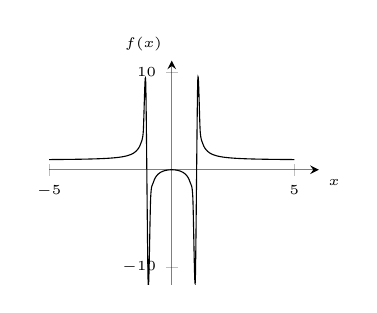
\begin{tikzpicture}
		    \begin{axis}[scale=.5,draw opacity =.5,samples=100,smooth, 
		      axis x line=center, 
		      axis y line=center,
		      ylabel = {$f(x)$},
		      xlabel = {$x$},
		      xlabel style={below right},
		      ylabel style={above left},
		      label style={font=\tiny},
		      tick label style={font=\tiny},
		      enlargelimits=upper] 
		      \addplot[black,opacity=1]{x^2/(x^2-1)};
		    \end{axis}
		\end{tikzpicture}
		\end{center}
		\vspace{.5cm}

	    %---------- (iv)
	    \item $f(x)=\dfrac{1}{1+x^2}$.\\\\
		Respuesta.-\;
		\begin{center}
		    \begin{tikzpicture}
		    \begin{axis}[scale=.5,draw opacity =.5,samples=100,smooth, 
		      axis x line=center, 
		      axis y line=center,
		      ylabel = {$f(x)$},
		      xlabel = {$x$},
		      xlabel style={below right},
		      ylabel style={above left},
		      label style={font=\tiny},
		      tick label style={font=\tiny},
		      enlargelimits=upper] 
		      \addplot[black,opacity=1]{1/(1+x^2)};
		    \end{axis}
		\end{tikzpicture}
		\end{center}
		\vspace{.5cm}
	\end{enumerate}

    %------------------ 4.
    \item 
	\begin{enumerate}[(a)]

	    %---------- (a)
	    \item Si $a_1<\ldots < a_n$ halle el valor mínimo de $f(x)=\sum\limits_{i=1}^n (x-a_i)^2$.\\\\
		Respuesta.-\; Primero calculamos la derivada de $f$.
		$$f'(x)=2(x-a_1)\cdot 1 + 2(x-a_2)\cdot 1 + \ldots + 2(x-a_n)\cdot 1=2\sum\limits_{i=1}^n (x-a_i).$$
		Luego encontremos los puntos críticos igualando $f'(x)$ cero.
		$$\begin{array}{rcl}
		    2\displaystyle\sum_{i=1}^n (x-a_i)=0 &\Rightarrow& (x-a_1)+(x-a_2)+\ldots + (x-a_n) = 0\\\\
							 &\Rightarrow& nx=a_1+a_2+\ldots + a_n\\\\
							 &\Rightarrow& x=\dfrac{1}{n}\displaystyle\sum_{i=1}^n a_i.
		\end{array}$$
		Veamos ahora si este punto crítico es un mínimo o un máximo local. Para ello calculamos la segunda derivada de $f$.
		$$\begin{array}{rcl}
		    f''(x)&=&2'\left[\displaystyle\sum_{i=1}^n (x-a_i)\right]+2\left[\displaystyle\sum_{i=1}^n (x-a_i)\right]'\\\\
			  &=&2(1+1+\ldots +1)\\\\
			  &=&2n.
		\end{array}$$
		Ya que $2n>0$, entonces podemos decir que el punto crítico $x=\dfrac{1}{n}\displaystyle\sum_{i=1}^n a_i$ es un mínimo local de $f$. Por lo tanto,
		$$f\left(\dfrac{1}{n}\sum_{i=1}^n a_i\right)=\sum_{i=1}^n \left[\dfrac{1}{n}\sum_{i=1}^n \left(a_i-a_i\right)\right]^2.$$\\

	    %---------- (b)
	    \item Halle ahora el valor mínimo de $f(x)=\sum\limits_{i=1}^n |x-a_i|$. Este es un problema en el que el cálculo infinitesimal no nos puede ayudar. En los intervalos entre los $a_i$ la función $f$ es lineal, por tanto el valor mínimo se localiza en uno de los $a_i$, y estos son, precisamente, los puntos en los cuales la función $f$ no es diferenciable. Sin embargo, la solución es fácil de encontrar si se considera como varía $f(x)$ al pasar de un intervalo a otro.\\\\
		Respuesta.-\; Tomemos dos puntos $a$ y $b$ en $[a_{i-1},a_i]$ y $[a_i,a_{i+1}]$ respectivamente. Tal que 
		$$|a-a_i|=|b-a_i|.$$
		Notemos que
		$$\begin{array}{rclr}
		    |b-a_j| &=& |a-a_j|+|a-b| & \mbox{si } j\leq i-1\\
		    |b-a_j| &=& |a-a_j|-|a-b| & \mbox{si } j\geq i+1
		\end{array}$$
		Luego, vemos que
		$$\begin{array}{rcl}
		    f(b) &=& \displaystyle \sum_{j=1}^n |b-a_j|\\\\
			 &=& \displaystyle \sum_{j=1}^{i-1} |b-a_j|+|b-a_i|+\sum_{j=i+1}^n|b-a_j|\\\\
			 &=& \displaystyle \sum_{j=1}^{i-1} \left(|a-a_j|+|a-b|\right)+|b-a_i|+\sum_{j=i+1}^n\left(|a-a_j|-|a-b|\right)\\\\
			 &=& \displaystyle \sum_{j=1}^{i-1} |a-a_j|+(i-1)|a-b|+|b-a_i|+\sum_{j=i+1}^n|a-a_j|-(n-i)|a-b|\\\\
			 &=& \displaystyle \sum_{j=1}^{i-1} |a-a_j|+|b-a_i|+\sum_{j=i+1}^n|a-a_j|(i-1)-(n-i)|a-b|\\\\
			 &=& \displaystyle \sum_{j=1}^{i-1} |a-a_j|+|b-a_i|+\sum_{j=i+1}^n|a-a_j|+(2i-n-1)|a-b|\\\\
		\end{array}$$
		Se sigue que $f(b)\geq f(a)$ siempre que
		$$2i-n-1\geq 0 \quad \mbox{o}\quad i\geq \dfrac{n+1}{2}.$$
		Por otro lado, de manera similar, $f(b)\leq f(a)$ siempre que
		$$2i-n-1\leq 0 \quad \mbox{o}\quad i\leq \dfrac{n+1}{2}.$$
		Así, tenemos a $f$ decreciente si $i\leq \dfrac{n+1}{2}$ y $f$ creciente si $i\geq \dfrac{n+1}{2}.$ De esta manera $f$ alcanza su mínimo en $a_{\frac{n+1}{2}}$ si $n$ es impar y está en el intervalo $\left[a_{\frac{n}{2}},a_{\frac{n}{2}+1}\right]$. Por lo tanto, el valor mínimo de $f$ es $f\left(a_{\frac{n+1}{2}}\right)$ si $n$ es impar y $f\left(a_{\frac{n}{2}}\right)$ si $n$ es par.\\\\

	    %---------- (c)
	    \item Sea $a>0$. Demuestre que el valor máximo de 
	    $$f(x)=\dfrac{1}{1+|x|}+\dfrac{1}{1+|x-a|}$$
	    es $(2+a)/(1+a)$. (Puede hallarse por separado la derivada en cada uno de los intervalos $(-\infty,0),(0,a)$ y $(a,\infty)$).\\\\
		Respuesta.-\; La función dada se puede escribir como sigue:
		$$f(x)=\left\{\begin{array}{rclcl}
			\dfrac{1}{1-x}+\dfrac{1}{1-x+a} &\mbox{si}& x<0\\\\
			\dfrac{1}{1+x}+\dfrac{1}{1-x+a} &\mbox{si}& 0<x<a\\\\
			\dfrac{1}{1+x}+\dfrac{1}{1+x-a} &\mbox{si}& x>a
		\end{array}\right.$$
		Notemos que $f$ es diferenciable en cada intervalo $(-\infty,0),(0,a)$ y $(a,\infty)$. Por lo que podemos hallar sus respectivas derivadas,
		$$f'(x)=\left\{\begin{array}{rclcl}
			\dfrac{1}{(1-x)^2}+\dfrac{1}{(1-x+a)^2} &\mbox{si}& x<0\\\\
			\dfrac{1}{(1+x)^2}+\dfrac{1}{(1-x+a)^2} &\mbox{si}& 0<x<a\\\\
			\dfrac{1}{(1+x)^2}+\dfrac{1}{(1+x-a)^2} &\mbox{si}& x>a
		\end{array}\right.$$
		el cual demuestra que $f'(x)>0$ si $(-\infty,0)$ y $f'(x)<0$ si $(a,\infty)$, esto ya que $(1-x)^2$ y $(1\pm x+a)^2$ son positivos. Además, vemos que
		$$f(0)=1+\dfrac{1}{1+a}=f(a)>0$$
		ya que $a>0.$ Así, $f$ es creciente en $(-\infty,0]$ y decreciente en $[a,\infty]$, donde se concluye que $f$ en $\mathbb{R}$ alcanza su punto máximo en algún punto del intervalo $[0,a]$. Ahora, verificamos si el máximo de $f$ se alcanza en algún punto en $(0,a)$. Si $b$ es tal punto, entonces 
		$$-\dfrac{1}{(1+b)^2}+\dfrac{1}{(1-b+a)^2}=0,$$
		el cual implica,
		$$(1+x)^2-(1-x+a)^2=(2+a)(2b-a)=0.$$
		Así, $b=\dfrac{a}{2}.$ Es más,
		$$f(0)=f(a)=1+\dfrac{1}{1+a}=\dfrac{2+a}{1+a}.$$
		Por lo tanto, se tiene que
		$$f\left(\dfrac{a}{2}\right)=\dfrac{2}{1+\dfrac{a}{2}}=\dfrac{4}{2+a}<\dfrac{2+a}{1+a}$$
		lo que muestra que $\dfrac{2+a}{1+a}$ es el máximo valor de $f$ en $[0,a]$.\\\\

	\end{enumerate}

    %-------------------- 5.
    \item Para cada una de las siguientes funciones, halle todos los puntos máximos y mínimos locales.
	\begin{enumerate}[(i)]

	    %---------- (i)
	    \item \;
	    $$f(x)=\left\{\begin{array}{rl}
		    x, & x\neq 3,5,7,9\\
		    5, & x=3\\
		    -3, & x=5\\
		    9, & x=7\\
		    7, & x=9
	    \end{array}\right.$$
	    \vspace{0.4cm}

		Respuesta.-\; Notemos que todos los puntos locales máximo y mínimos deben estar en el conjunto $\left\{3,5,7,9\right\}$, ya que, aparte de estos puntos, $f$ cumple la función identidad. Ahora vemos por la definición de $f$ que 
		\begin{center}
		    $f(3)=5>3$ y $5>x$, para todo $x\in (3-\delta,3+\delta)$, para $0<\delta<1.$
		\end{center}
		Así, $3$ es un punto máximo local.\\

		Para $x=5$ tenemos por la definición de $f$ que
		\begin{center}
		    $f(5)=-3<x$ para todo $x\geq 0.$
		\end{center}
		Así, $5$ es un punto mínimo local.\\

		También vemos por la definición de $f$ que
		\begin{center}
		    $f(7)=9>7$ y $9>x$, para todo $x\in (7-\delta,7+\delta)$, para $0<\delta<1.$
		\end{center}
		Así, $7$ es un punto máximo local.\\

		Para $x=5$ tenemos por la definición de $f$ que
		\begin{center}
		    $f(9)=7<9$ y $7<x,$ para todo $x\in (9-\delta,9+\delta)$, para $0<\delta<1.$
		\end{center}
		Así, $9$ es un punto mínimo local.\\\\

	    %---------- (ii)
	    \item \;
	    $$f(x)=\left\{\begin{array}{rl}
		    0, & x \mbox{ irracional}\\
		    1/q, & x=p/q \mbox{ fracción irreducible}.
	    \end{array}\right.$$
	    \vspace{0.4cm}

		Respuesta.-\; Notemos que cada número irracional $x$ es un mínimo local de $f$ ya que , en el caso de que $f(x)=0$ y $f(y)=\dfrac{1}{q}>0,$ para cualquier racional $y=p/q$. Por otro lado, no existe un punto máximo local. De hecho, vemos por la definición de $f$ que el máximo local sólo puede ocurrir para los números racionales. Pero para cualquier racional $x=p/q$, $f(x)=1/q<p/q=x$ si $p>0$ y $f(x)=1/q>p/q=x$  si $p<0$ pero $f(x)>0=f(y)$, para cualquier número racional $y$.\\\\

	    %---------- (iii)
	    \item \;
	    $$f(x)=\left\{\begin{array}{rl}
		    x,& x \mbox{ racional}\\
		    0, x& \mbox{ irracional}.
	    \end{array}\right.$$
	    \vspace{0.4cm}

		Respuesta.-\; Observamos que todo número irracional positivo $x$ es un mínimo local de $f$. Ya que, en este caso, $f(x)=0$ y $f(y)=y>0$, para cualquier racional $y\geq0$. Por otro lado, para cualquier racional $y\leq 0$, tenemos $f(y)=y\leq 0$ y por lo tanto cualquier número irracional estrictamente negativo es un máximo local de $f$.\\\\

	    %---------- (iv)
	    \item \;
	    $$f(x)=\left\{\begin{array}{rl}
		    1, & x=1/n \mbox{ para algún } n\in \mathbb{N}\\
		    0, &x \mbox{ en los demás casos}.
	    \end{array}\right.$$
	    \vspace{0.4cm}

	    Respuesta.-\; Notemos que, para cada $n\in \mathbb{N}, 1/n$ es un punto local máximo a partir de la definición de $f$, $f(\frac{1}{n})=1,$ y $f(x)=0.$ Similarmente, vemos que para cada número real tal que $\left\{\frac{1}{n}:n\in \mathbb{N}\right\}$ es un punto mínimo local, ya que en este conjunto $f$ es idénticamente $0$. Además si $f$ es constante para cada número real tal que $\left\{\frac{1}{n}:n\in \mathbb{N}\right\}$, entonces es un punto máximo y mínimo local a la vez, excepto el punto $0$, ya que para cada $\epsilon>0$, $(-\delta, \delta)$ contiene infinitos $1/n$, esto por la propiedad Arquimediana de los números reales.\\\\

	    %---------- (v)
	    \item \;
	    $$f(x)=\left\{\begin{array}{rl}
		    1, & x \mbox{ si el desarrollo decimal de } x \mbox{contiene un } 5\\
		    0, &x \mbox{ en los demás casos}.
	    \end{array}\right.$$
	    \vspace{0.4cm}

		Respuesta.-\; Notemos que para cada
		$$x\in \left\{x\in \mathbb{R}:\mbox{el desarrollo decimal de } x \mbox{contiene a } 5\right\}$$
		es un punto máximo local a partir de la definición de $f$. Es este caso, $f(x)=1$ y $f$ es $0$. Similarmente, vemos que cada número real tal que, 
		$$\left\{x\in \mathbb{R}:\mbox{el desarrollo decimal de } x \mbox{contiene a } 5\right\}$$
		es un punto mínimo local, ya que en este conjunto $f$ es idénticamente $0$. Además, ya que $f$ es constante, tenemos que cada número en el conjunto 
		$$\left\{x\in \mathbb{R}:\mbox{el desarrollo decimal de } x \mbox{contiene a } 5\right\}$$
		es un punto máximo local y un punto mínimo local, excepto el punto $0$, ya que para cada $\delta>0,$ $(-\delta,\delta)$ contiene infinitos puntos con al menos un $5$ en su expansión decimal, esto por la propiedad Arquimediana de los números reales\\\\

	\end{enumerate}

    %-------------------- 6.
    \item Demuestre la siguiente propiedad (que se utiliza muchas veces de manera implícita): si $f$ es creciente en $(a, b)$ y continua en $a$ y $b$, entonces $f$ es creciente en $[a, b]$. En particular, si $f$ es continua en $[a, b]$ y $f > 0$ en $(a, b)$, entonces $f$ es creciente en $[a, b]$.\\\\
	Demostración.-\; Sea $x,y\in [a,b]$ tal que x<y. Ya que $f$ es creciente en $(a,b)$, entonces $f$ es también creciente en $(x,y)$. Por el teorema de valor medio, existe un $c\in (x,y)$ tal que 
	$$f(y)-f(x)=f'(c)(y-x)>0.$$
	Si $f$ es creciente en $(x,y)$,
	$$f'(c)\geq 0 \mbox{ para todo } c\in (x,y).$$
	Por el hecho de que $y-x>0$, entonces
	$$f(x)<f(y).$$
	De esta manera, $x$ e $y$ son número arbitrarios en $[a,b]$ y por lo tanto $f$ es creciente en $[a,b]$.\\\\

    %-------------------- 7.
    \item Se traza una recta desde el punto $(0, a)$ hasta el eje horizontal y desde allí otra a $(1, b)$, tal como se indica en la Figura 23 (Spivak). Demuestre que la longitud total es mínima cuando los ángulos $\alpha$ y $\beta$ son iguales. (Naturalmente, deberá entrar en juego una función: expresar la longitud en términos de $x$, donde $(x, 0)$ es el punto del eje horizontal. La línea a trazos de la Figura 23 sugiere una demostración geométrica; tanto en un caso como en otro puede resolverse el problema sin necesidad de hallar el punto $(x, 0)$.)\\\\
	Demostración.-\; De la figura dada, encontramos que la longitud total del camino está dada por: 
	$$f(x)=\sqrt{x^2+a^2}+\sqrt{(1-x)^2+b^2}.$$
	Para la longitud más corta, obtenemos la primera derivada y la igualamos con cero
	$$\dfrac{x}{\sqrt{x^2+a^2}}-\dfrac{1-x}{\sqrt{(1-x)^2+b^2}}=0.$$
	Reemplazando $\dfrac{x}{\sqrt{x^2+a^2}}$ con $\cos \alpha$ y $\dfrac{1-x}{\sqrt{(1-x)^2+b^2}}$ con $\cos \beta$, obtenemos
	$$\cos \alpha-\cos \beta=0 \quad \Rightarrow \quad \cos \alpha = \cos \beta \quad \Rightarrow \quad \alpha = \beta.$$\\

    %-------------------- 8.
    \item 
	\begin{enumerate}[(a)]

	    %---------- (a)
	    \item Sea $(x_0,y_0)$ un punto del plano, y sea $L$ la gráfica de la función $f(x)=mx+b.$ Halle el punto $\overline{x}$ tal que la distancia de $(x_0,y_0)$ a $(\overline{x},f(\overline{x}))$ sea mínima. [Observe que minimizar esta distancia equivale a minimizar su cuadrado. Esto puede simplificar, en cierta medida, los cálculos.]\\\\
		Respuesta.-\; La distancia entre $(x_0,y_0)$ y algún punto $x$ que satisfaga $f(x)=mx+b$ es:
		$$d^2=\left(x_0-x\right)^2+\left(y_0-mx-b\right)^2$$
		Derivando a ambos lados con respecto a $x$, 
		$$2dd'=-2\left(x_0-x\right)+2m\left(y_0+mx-b\right)$$
		Por la distancia más corta, entonces $d'=0$. Luego,
		$$-x_0+x-my_0+m^2x+bm=0 \quad \Rightarrow \quad x=\dfrac{x_0+my_0-bm}{m^2+1}.$$\\

	    %---------- (b)
	    \item Halle también $\overline{x}$ observando que la recta que va de $(x_0.y_0)$ a $\left(\overline{x},f(\overline{x})\right)$ es perpendicular a $L$.\\\\
		Respuesta.-\; La distancia más corta ocurre cuando la linea de $(x_0,y_0)$ es perpendicular a $L$,
		$$x=\dfrac{x_0+my_0-bm}{m^2+1}.$$\\

	    %---------- (c)
	    \item Halle la distancia de $(x_0,y_0)$ de $L$. Es decir, la distancia de $(x_0,y_0)$ a $\left(\overline{x},f(\overline{x})\right)$. [Facilitará los cálculos suponer primero que $b=0$; luego aplicar el resultado a la gráfica de $f(x)=mx+b$ y el punto $(x_0,y_0-b)$].\\\\
		Respuesta.-\; Sea la ecuación dada en el inciso (a),
		$$d=\sqrt{\left(x_0-x\right)^2+\left(y_0-mx-b\right)^2}.$$
		Supongamos $b=0$, entonces
		$$d=\sqrt{x_0^2-2x_0x+x^2+y_0^2-2my_0x+m^2x^2}\quad \Rightarrow \quad d=\sqrt{\left(m^2+1\right)x^2-2\left(x_0+my_0\right)x+x_0^2+y_0^2}.$$
		Reemplazando $x$ con $\dfrac{x_0+my_0}{m^2+1}$,
		$$\begin{array}{rcl}
		    d&=&\sqrt{\left(\dfrac{x_0+my_0}{m^2+1}\right)^2-2\dfrac{\left(x_0+my_0\right)^2}{m^2+1}+x_0^2+y_0^2}\\
		     &=&\sqrt{-\dfrac{\left(x_0+my_0\right)^2}{m^2+1}+x_0^2+y_0^2}\\\\
		     &=&\sqrt{\dfrac{-x_0^2-2mx_0y_0-m^2y_0^2+x_0^2m^2+y_0^2m^2+x_0^2+y_0^2}{m^2+1}}\\\\
		     &=&\sqrt{\dfrac{\left(y_0-mx_0\right)^2}{m^2+1}}\\\\
		\end{array}$$
		Reemplazando $y_0$ con $y_0-b$, concluimos que,
		$$\begin{array}{rcl}
		    d&=&\dfrac{\left(y_0-b-mx_0\right)^2}{m^2+1}\\\\
		     &=&\dfrac{y_0-b-mx_0}{\sqrt{m^2+1}}
		\end{array}$$
		\vspace{0.5cm}\\\\

	    %---------- (d)
	    \item Considere una recta descrita mediante la ecuación $Ax+By+C=0$. Demuestre que la distancia de $\left(x_0,y_0\right)$ a esta recta es $\left(Ax_0+By_0+C\right)/\sqrt{A^2+B^2}$.\\\\
		Demostración.-\; Sea la ecuación:
		$$Ax+By+C=0$$
		de donde, encontrar la pendiente $m=-\dfrac{A}{B}.$
		Substituyendo en la ecuación de la parte (c), se tiene
		$$d=\dfrac{y_0-b+\dfrac{A}{B}x_0}{\sqrt{\left(-\dfrac{A}{B}\right)^2}+1}$$
		Luego, multiplicando ambos lados por $\dfrac{B}{B}$,
		$$\begin{array}{rcll}
		    d&=&\dfrac{Ax_0+By_0-bB}{\sqrt{A^2+B^2}}&\\\\
		     &=&\dfrac{Ax_0+By_0+C}{\sqrt{A^2+B^2}}&\mbox{supongamos } bB=-C.
		\end{array}$$
		\vspace{0.5cm}\\\\

	\end{enumerate}

    %-------------------- 9.
    \item El problema anterior (8, Michael Spivak, capítulo 11) sugiere la siguiente cuestión: ¿cuál es la relación entre los puntos críticos de $f$ y los de $f^2$?.\\\\
	Respuesta.-\; Los puntos críticos de una función son los puntos en los que la función no es diferenciable o su primera derivada es cero. Sabemos que para definir los puntos críticos se iguala  $f'$ a cero y para los puntos críticos podemos igualar también $\left(f^2\right)'$ a cero, lo que implica
	$$\left(f^2\right)'=2ff'$$
	Por lo tanto, los puntos críticos de $f$ son subconjuntos de los puntos críticos de $f^2$.\\\\

    %-------------------- 10.
    \item Demuestre que entre todos los rectángulos de igual perímetro, el de mayor área es el cuadrado.\\\\
	Demostración.-\; Sean $l$ el largo, $a$ el ancho y $p$ el perímetro del rectángulo. Entonces,
	$$p=2(l+a)\quad \Rightarrow \quad a=\dfrac{p}{2}-l.$$
	Sabemos que el área, llamémosla $A$, está dada por:
	$$A=l \cdot a$$
	De donde,
	$$A=l\left(\dfrac{p}{2}-l\right)=\dfrac{p}{2}l-l^2.$$
	Derivando con respecto a $l$, se tiene
	$$A'=\dfrac{p}{2}-2l.$$
	Luego igualando a cero, se tiene
	$$\dfrac{p}{2}-2l=0\quad \Rightarrow \quad l=\dfrac{p}{4}.$$
	Por el corolario 11.3 y sabiendo que si $f'<0$ en $\left(-\infty,\frac{p}{4}\right)$  y $f'>0$ en $\left(\frac{p}{4},\infty\right)$. Entonces, $\frac{p}{4}$ es un punto mínimo local.\\

	Luego, reemplazando $l=\frac{p}{4}$ en $a=\frac{p}{2}-l$, se tiene
	$$a=\dfrac{p}{2}-\frac{p}{4}=l.$$
	Por lo tanto, el área del rectángulo es la más pequeña cuando su largo es igual a su ancho y se convierte en un cuadrado.\\\\

    %-------------------- 11.
    \item Entre todos los cilindros circulares rectos de volumen fijo $V$, halle el de menor superficie (incluyendo las superficies de las caras superior e inferior como en la Figura 24, Spivak, capítulo 11.).\\\\
	Respuesta.-\; El volumen $V$ de un cilindro con radio $r$ y altura $h$ es:
	$$V=\pi r^2h \quad \Rightarrow \quad h=\dfrac{V}{\pi r^2}.$$
	Luego, el área total $A$ de un cilindro está dada por:
	$$A=2\pi r^2+2\pi rh.$$
	Reemplazado $h$  en esta ecuación, se tiene
	$$A=2\pi r^2+2\pi r\dfrac{V}{\pi r^2}=2\pi r^2+\dfrac{2V}{r}.$$
	Derivando con respecto a $r$, se tiene
	$$A'=4\pi r - \dfrac{2V}{r^2}.$$
	Luego igualando a cero,
	$$4\pi r - \dfrac{2V}{r^2}=0\quad \Rightarrow \quad r=\dfrac{V}{\pi\left(\sqrt[3]{\dfrac{V}{2\pi}}\right)^2}.$$
	Por el corolario 11.3 y sabiendo que si $f'<0$ en $\left(-\infty,\dfrac{V}{\pi\left(\sqrt[3]{\dfrac{V}{2\pi}}\right)^2}\right)$  y $f'>0$ en $\left(\dfrac{V}{\pi\left(\sqrt[3]{\dfrac{V}{2\pi}}\right)^2},\infty\right)$. Entonces, $\dfrac{V}{\pi\left(\sqrt[3]{\dfrac{V}{2\pi}}\right)^2}$ es un punto mínimo local.\\
	Reemplazando $r$ en $h=\dfrac{V}{\pi r^2}$, obtenemos 
	$$h=\dfrac{V}{\pi\pi\left(\sqrt[3]{\dfrac{V}{2\pi}}\right)^2}.$$
	Por lo tanto, el área superficial del cilindro es la más pequeña cuando su radio es $\sqrt[3]{\dfrac{V}{2\pi}}$ y su altero es $\dfrac{V}{\pi\pi\left(\sqrt[3]{\dfrac{V}{2\pi}}\right)^2}$.\\\\

    %-------------------- 12.
    \item Un triángulo rectángulo cuya hipotenusa tiene una longitud $a$ gira alrededor de uno de sus lados, generando un cono circular recto. Halle el volumen máximo que puede tener este cono.\\\\
	Respuesta.-\; El volumen $V$ de un cono con radio $r$ y alguna altura $h$ es:
	$$V=\dfrac{1}{3}\pi r^2 h.$$
	Aplicando el teorema de Pitágoras,
	$$a^2=r^2+h^2 \quad \Rightarrow \quad h=\sqrt{a^2-r^2}.$$
	Reemplazando en $V=\dfrac{1}{3}\pi r^2 h$, se tiene
	$$V=\dfrac{1}{3}\pi r^2 \sqrt{a^2-r^2}\quad \Rightarrow\quad V=\dfrac{1}{3}\pi\sqrt{r^4a^2-r^6}.$$
	Derivando con respecto a $r$, 
	$$V'=\dfrac{1}{3}\pi\dfrac{4r^3a^2-6r^5}{\sqrt{r^4a^2-r^6}}.$$
	Luego igualando a cero,
	$$\dfrac{4r^3a^2-6r^5}{\sqrt{r^4a^2-r^6}}=0\quad \Rightarrow \quad 2a^2-3r^2=0 \quad \Rightarrow \quad r=\sqrt{\dfrac{2}{3}}a.$$
	Reemplazando $r$ en $V=\dfrac{1}{3}\pi r^2 h$, obtenemos 
	$$V=\dfrac{1}{3}\pi\sqrt{\dfrac{4}{9}a^6-\dfrac{8}{27}a^6}=\dfrac{1}{3}\pi\sqrt{\dfrac{4}{27}}a^6=\dfrac{2\sqrt{3}\pi}{27}a^3.$$
	El cual es el mayor volumen.\\\\

    %-------------------- 13.
    \item Demuestre que la suma de un número positivo y de su recíproco es al menos $2$.\\\\
	Demostración.-\; Sean $a$ un número positivo y $\dfrac{1}{a}$ para $a\neq 0$ es su reciproco. Definamos la suma $sum$ de estos dos números, como sigue
	$$sum=a+\dfrac{1}{a}.$$
	Derivando con respecto a $a$,
	$$sum'=1-\dfrac{1}{a^2}.$$
	Luego igualando a cero,
	$$1-\dfrac{1}{a^2}=0\quad \Rightarrow \quad a^2=1 \quad \Rightarrow \quad a=\pm 1.$$
	Ya que $a$ es un número positivo, solo se evaluará en $a=1$. Por el corolario 11.3, y sabiendo que si $sum'<0$ cuando $(0,1)$ y $sum'>0$ cuando $(1,\infty)$. Es decir $sum$ es decreciente cuando $(0,1)$ y creciente cuando $(1,\infty)$. Entonces $a$ es un punto mínimo. Luego reemplazando $a$ en $sum=a+\dfrac{1}{a}$ se tiene,
	$$sum=1+1=2.$$\\

    %-------------------- 14.
    \item Halle el trapezoide de mayor área que puede ser inscrito en un semicírculo de radio $a$, con una base situada a lo largo del diámetro.\\\\
	Respuesta.- \; Tracemos primero una gráfica.
	\begin{center}
	    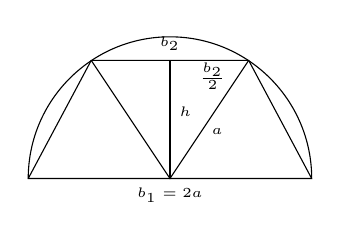
\begin{tikzpicture}[baseline=(current bounding box.north)]
	      \def\Radius{1.8}
	      \path
		(-\Radius, 0) coordinate (A)
		-- coordinate (M)
		(\Radius, 0) coordinate (B)
		(M) +(60:\Radius) coordinate (C)
		+(120:\Radius) coordinate (D)
	      ;
	      % Draw semicircle
		  \draw
		    (B) arc(0:180:\Radius) -- cycle
		  ;
		  % Annotations
		  \path[inner sep=0pt];
		  \draw(-1.8,0)--(-1,1.5)--(1,1.5)--(1.8,0);
		  \draw(0,0)--(0,1.5)node[above]{\tiny$b_2$};
		  \draw(1,1.5)--(0,0)node[below]{\tiny$b_1=2a$}--(-1,1.5);
		  \draw(.6,.6)node[]{\tiny$a$};
		  \draw(0,.85)node[right]{\tiny$h$};
		  \draw(.25,1.3)node[right]{\tiny$\frac{b_2}{2}$};
	    \end{tikzpicture}
	\end{center}

	Por la esta figura, tenemos:
	$$b_2=2\sqrt{a^2-h^2}.$$
	Sabemos que el área del trapezoide está dado por:
	$$A=\dfrac{1}{2}(b_1+b_2)h.$$
	Reemplazando $b_1$ con $2a$ y $b_2$ con $2\sqrt{a^2-h^2}$, se tiene:
	$$\begin{array}{rcl}
	    A&=&\dfrac{1}{2}\left(2a+2\sqrt{a^2-h^2}\right)h\\\\
	     &=&ah+\sqrt{a^2h^2-h^4}.
	\end{array}$$
	Derivando con respecto a $x$,
	$$\begin{array}{rcl}
	    A'&=&a+\dfrac{2a^2h-4h^3}{2\sqrt{a^2h^2-h^4}}\\\\
	      &=&\dfrac{a\sqrt{a^2h^2-h^4}+a^2h-2h^3}{\sqrt{a^2h^2-h^4}}.
	\end{array}$$
	Luego igualando a cero,
	$$\begin{array}{rcl}
	    a\sqrt{a^2h^2-h^4}+a^2h-2h^3&=&0\\\\
	    a\sqrt{a^2-h^2}+a^2-2h^2&=&0\\\\
	    a^2\left(a^2-h^2\right) &=& 4h^4-4a^2h^2+a^4\\\\
	    h&=&\dfrac{\sqrt{3}}{2}a
	\end{array}$$

	Evaluando $h$ en $A=ah+\sqrt{a^2h^2-h^4}$, obtenemos:
	$$\begin{array}{rcl}
	    A&=&\dfrac{\sqrt{3}}{2}a^2+\sqrt{\dfrac{3}{4}a^4-\dfrac{9}{16}a^4}\\\\
	     &=&\dfrac{\sqrt{3}}{2}a^2+\dfrac{\sqrt{3}}{4}a^2\\\\
	     &=&\dfrac{3\sqrt{3}}{4}a^2
	\end{array}.$$
	\vspace{.5cm}

    %-------------------- 15.
    \item Dos pasillos de anchuras $a$ y $b$, forman un ángulo recto (Figura 25,Spivak, capítulo 11). ¿Cuál es la longitud máxima de una escalera que puede ser transportada horizontalmente alrededor de la esquina?.\\\\
	Respuesta.-\; Por la figura dada, tenemos:
	$$\sen \theta = \dfrac{b}{x}\quad \Rightarrow \quad x=\dfrac{b}{\sen \theta}.$$
	Y
	$$\cos \theta = \dfrac{a}{L-x}\quad \Rightarrow \quad L-x=\dfrac{a}{\cos \theta}.$$
	De donde, reemplazando la primera ecuación en la segunda, se tiene:
	$$L=\dfrac{a}{\cos \theta}+\dfrac{b}{\sen \theta}.$$
	Derivando con respecto a $\theta$,
	$$\begin{array}{rcl}
	    L'&=&\dfrac{a\sen \theta}{\cos^2\theta}-\dfrac{b\cos \theta}{\sen^2 \theta}\\\\
	      &=&\dfrac{a\sen^3\theta-b\cos^3\theta}{\cos^2\theta\sen^2\theta}.
	\end{array}$$
	Para la mayor longitud posible, igualamos $L'$ a cero,
	$$\begin{array}{rcl}
	    a\sen^3\theta-b\cos^3\theta&=&0\\\\
	    a\sen^3\theta&=&b\cos^3\theta\\\\
	    \dfrac{\sen^3\theta}{\cos^3\theta}&=&\dfrac{b}{a}\\\\
	    \tan^3\theta&=&\dfrac{b}{a}\\\\
	    \tan \theta &=& \sqrt[3]{\dfrac{b}{a}}\\\\
	    \sen\theta &=&\dfrac{\sqrt[3]{\dfrac{b}{a}}}{\sqrt{1+\left(\sqrt[3]{\dfrac{b}{a}}\right)^2}}\\\\
	    \cos\theta &=& \dfrac{1}{\sqrt{1+\left(\sqrt[3]{\dfrac{b}{a}}\right)^2}}\\\\
	\end{array}$$
	Reemplazando los valores de $\sen$ y $\cos$ en $L=\dfrac{a}{\cos \theta}+\dfrac{b}{\sen \theta}$, para obtener la mayor longitud posible, se tiene:
	$$L=a\sqrt{1+\left(\sqrt[3]{\dfrac{b}{a}}\right)^2}+b\dfrac{\sqrt{1+\left(\sqrt[3]{\dfrac{b}{a}}\right)^2}}{\sqrt[3]{\dfrac{b}{a}}}.$$\\

    %-------------------- 16.
    \item Se diseña un jardín en forma de un sector circular (Figura 26, Spivak, capítulo 11), de radio $R$ y ángulo central $\theta$ . El jardín debe tener un área fija $A$. ¿Para qué valor de $R$ y $\theta$ (en radianes) será mínima la longitud de la valla alrededor del perímetro del jardín?.\\\\
	Respuesta.-\; El área del jardín es:
	$$A=\dfrac{1}{2}r^2\theta\quad \Rightarrow \quad \theta=\dfrac{2A}{r^2}.$$
	Después, el perímetro del jardín está dado por:
	$$P=r\theta+2r.$$
	Luego, reemplazando por $\theta=\dfrac{2A}{r^2}$:
	$$P=\dfrac{2A}{r}+2r.$$
	Derivando con respecto a $r$,
	$$P'=\dfrac{-2A}{r^2}+2.$$
	Para hallar el valor de $r$ que minimiza $P$, igualamos $P'$ a cero,
	$$\begin{array}{rcl}
	    \dfrac{-2A}{r^2}+2&=&0\\\\
	    \dfrac{2A}{r^2}&=&-2\\\\
	    r^2&=&A\\\\
	    r&=&\sqrt{A}.
	\end{array}$$
	Reemplazando en $\theta=\dfrac{2A}{r^2}$, se tiene:
	$$\theta=\dfrac{2A}{(\sqrt{A})^2}=\dfrac{2A}{A}=2.$$\\

    %-------------------- 17.
    \item Un ángulo recto se desplaza a lo largo del diámetro de un círculo de radio a, tal como se muestra en la Figura 27 (Spivak, Capítulo 11). ¿Cuál es la mayor longitud posible $(A + B)$ interceptada por el círculo sobre el ángulo?.\\\\
	Respuesta.-\; Complementando el dibujo dado, podríamos construir:
	\begin{center}
	    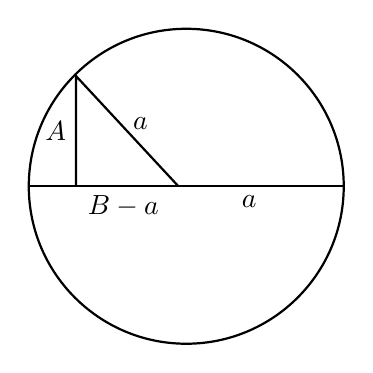
\begin{tikzpicture}[scale=1]
		\draw[thick] (0,0) circle (2);
		\draw[thick] (-2,0) -- (2,0);
		\draw[thick] (-1.4,0) -- (-1.4,1.4)--(-.1,0);
		\draw(-1.4,0.7)node[left]{$A$};
		\draw(-.8,0)node[below]{$B-a$};
		\draw(-.8,1)node[below right]{$a$};
		\draw(.8,0)node[below]{$a$};
	    \end{tikzpicture}
	\end{center}
	Donde podemos definir lo siguiente:
	$$A=\sqrt{a^2-(B-a)^2}=\sqrt{2aB-B^2}$$
	$$S=A+B=\sqrt{2aB-B^2}+B.$$
	Derivando con respecto a $B$,
	$$S'=\dfrac{2a-2B}{\sqrt{2aB-B^2}}+1.$$
	Para la mayor longitud posible, igualamos $S'$ a cero,
	$$\begin{array}{rcl}
	    \dfrac{2a-2B}{2\sqrt{2aB-B^2}}&=&0\\\\
	    B-a&=&\sqrt{2aB-B^2}\\\\
	    B^2-2aB+a^2&=&2aB-B^2\\\\
	    2B^2-4aB+a^2&=&0\\\\
	    B&=&\dfrac{4a\pm \sqrt{16a^2-4\cdot 2a^2}}{2\cdot 2}\\\\
	    B&=&\dfrac{2a\pm \sqrt{2}a}{2}=\left(1+\pm \dfrac{\sqrt{2}}{2}\right)a.
	\end{array}$$
	Luego, sea $B=a\left(1+\dfrac{\sqrt{2}}{2}\right)$, entonces reemplazando en $A=\sqrt{2aB-B^2}$, se tiene
	$$\begin{array}{rcl}
	    A&=&\sqrt{2a^2\left(1+\dfrac{\sqrt{2}}{2}\right)-\left[a\left(1+\dfrac{\sqrt{2}}{2}\right)\right]^2}\\\\
	    A&=&\dfrac{\sqrt{2}a}{2}.
	\end{array}$$
	Sea ahora $B=a\left(1-\dfrac{\sqrt{2}}{2}\right)$, entonces reemplazando en $A=\sqrt{2aB-B^2}$, se tiene
	$$\begin{array}{rcl}
	    A&=&\sqrt{2a^2\left(1-\dfrac{\sqrt{2}}{2}\right)-\left[a\left(1-\dfrac{\sqrt{2}}{2}\right)\right]^2}\\\\
	    A&=&\dfrac{\sqrt{2}a}{2}.
	\end{array}$$
	\vspace{.5cm}

    %-------------------- 18.
    \item El ecólogo Ed debe cruzar un lago circular de $1$ milla de radio. Puede remar a través del lago a una velocidad de $2$ millas por hora, o caminar alrededor del lago a una velocidad de $4$ millas por hora; también puede remar un cierto trecho y completar el itinerario caminando (Figura 28, Spivak, capítulo 11). ¿Qué ruta debe tomar de manera que:

	\begin{enumerate}[(i)]

	    %---------- (i)
	    \item pueda ver la mayor cantidad de paisaje posible?.\\\\
		Respuesta.-\; Sea,
		\begin{center}
		    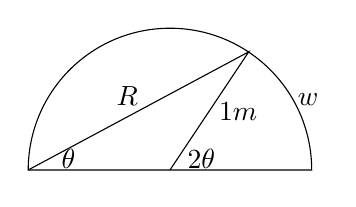
\begin{tikzpicture}[baseline=(current bounding box.north)]
		      \def\Radius{1.8}
		      \path
			(-\Radius, 0) coordinate (A)
			-- coordinate (M)
			(\Radius, 0) coordinate (B)
			(M) +(60:\Radius) coordinate (C)
			+(120:\Radius) coordinate (D)
		      ;
		      % Draw semicircle
			  \draw
			    (B) arc(0:180:\Radius) -- cycle
			  ;
			  % Annotations
			  \path[inner sep=0pt];
			  \draw(-1.8,0)--(1,1.5)--(0,0);
			  \draw(-1.5,-.1)node[above right]{$\theta$};
			  \draw(-.8,.7)node[above right]{$R$};
			  \draw(.1,-.1)node[above right]{$2\theta$};
			  \draw(.5,.5)node[above right]{$1m$};
			  \draw(1.5,.7)node[above right]{$w$};
		    \end{tikzpicture}
		\end{center}
		Sea $R$ que representa la distancia que el hombre recorrerá y $W$ la distancia que caminerá como se muestra en la figura anterior, de donde
		$$W=2r\theta = 2\theta$$
		Y
		$$R^2=1^2+1^2=-2\cdot 1\cdot 1 \cdot \cos(\pi-2\theta).$$
		Aplicando la identidad trigonométrica $\cos(\pi - \theta)=-\cos(\theta)$,
		$$R^2=2+2\cos(2\theta)\quad \Rightarrow \quad R=\sqrt{2+2\cos(2\theta)}.$$
		Luego, la longitud $D$ del camino total viene dada por:
		$$D=R+W=2\theta+\sqrt{2+2\cos(2\theta)}.$$
		Derivando con respecto a $\theta$,
		$$D'=2-\dfrac{4\sen(2\theta)}{2\sqrt{2+2\cos(2\theta)}}$$
		Para hallar la mayor longitud posible, igualamos $D'$ a cero,
		$$\begin{array}{rclr}
		    2-\dfrac{4\sen(2\theta)}{2\sqrt{2+2\cos(2\theta)}}&=&0&\\\\
		    \dfrac{\sen(2\theta)}{\sqrt{2+2\cos(2\theta)}}&=&1&\\\\
		    \sen(2\theta)&=&\sqrt{2+2\cos(2\theta)}&\\\\
		    \sen^2(2\theta)&=&2+2\cos(2\theta)&\\\\
			1-\cos^2(2\theta)-2\cos(2\theta)+1&=&0&\sen^2(\theta)=1-\cos^2(\theta)\\\\
							  \cos^2(2\theta)+2\cos(2\theta)+1&=&0&\\\\
							  \left[\cos(2\theta)+1\right]^2&=&0&\\\\
							  \cos(2\theta)&=&-1&\\\\
							  2\theta&=&\pi&2\theta=\arccos(-1)\\\\
							  \theta&=&\dfrac{\pi}{2}&
		\end{array}$$
		Reemplazando $\theta=\dfrac{\pi}{2}$ en $W=2\theta$ y $R=\sqrt{2+2\cos(2\theta)}$ se tiene
		$$W=\pi \qquad \mbox{y}\qquad R=\sqrt{2+2\cos(\pi)}=0.$$\\\\

	    %---------- (ii)
	    \item pueda cruzar tan rápida como sea posible?
		Respuesta.-\; Aplicando la fórmula,
		$$tiempo=\dfrac{distancia}{velocidad}$$
		Se tiene que el tiempo total es:
		$$T=\dfrac{W}{4}+\dfrac{R}{2}.$$
		Reeemplazando $W$ con $2\theta$ y $R$ con $\sqrt{2+2\cos(2\theta)}$,
		$$T=\dfrac{\theta}{2}+\dfrac{1}{2}\sqrt{2+2\cos(2\theta)}.$$
		Derivando con respecto a $\theta$,
		$$T'=\dfrac{1}{2}-\dfrac{\sen(2\theta)}{\sqrt{2+2\cos(2\theta)}}.$$
		Para el tiempo mínimo, igualamos $T'$ a cero,
		$$\begin{array}{rclr}
		    \dfrac{1}{2}-\dfrac{\sen(2\theta)}{\sqrt{2+2\cos(2\theta)}}&=&0&\\\\
		    2\sen(2\theta)&=&\sqrt{2+2\cos(2\theta)}&\\\\
		    4\sen^2(2\theta)&=&2+2\cos(2\theta)&\\\\
		    4-4\cos^2(2\theta)-2\cos(2\theta)-2&=&0&\sen^2(\theta)=1-\cos^2(\theta)\\\\
		    2\left[2-2\cos^2(2\theta)-\cos(2\theta)-1\right]&=&0\\\\
		    \left[2\cos(2\theta)-1\right]\left[\cos(2\theta)+1\right]&=&0&\\\\
		    \cos(2\theta)=\dfrac{1}{2}&\mbox{o}&\cos(2\theta)=-1&\\\\
		    2\theta=\arccos\left(\dfrac{1}{2}\right)&\mbox{o}&2\theta=\arccos(-1)&\\\\
		    \theta=\dfrac{\pi}{6}&\mbox{o}&\theta=\dfrac{\pi}{2}&
		\end{array}$$

		Para $\theta=\dfrac{\pi}{6},$
		$$W=\dfrac{\pi}{3}\qquad \mbox{y}\qquad R=\sqrt{2+2\cos\left(\dfrac{\pi}{3}\right)}=\sqrt{3}.$$
		Por lo tanto,
		$$T=\dfrac{\pi}{12}+\dfrac{\sqrt{3}}{2}.$$

		Para $\theta=\dfrac{\pi}{2},$
		$$W=\pi \qquad \mbox{y}\qquad R=\sqrt{2+2\cos(\pi)}=0.$$
		Por lo tanto,
		$$T=\dfrac{\pi}{4}.$$\\

	\end{enumerate}


    %-------------------- 19.
    \item 
	\begin{enumerate}[(a)]

	    %---------- (a)
	    \item Considere los puntos $A$ y $C$ de un círculo, con cetro $O$, formando un ángulo $\alpha=\angle AOC$ (figura 29, Spivak, capítulo 11). ¿Cómo debe elegirse el punto $B$ de manera que la suma de las áreas del triángulo $\triangle AOB$ y del triángulo $\triangle BOC$ sea máxima? Indicación: Exprese todo en función de $\theta = \angle AOB.$\\\\
		Respuesta.-\; La suma de las áreas de los dos triángulos es:
		$$\begin{array}{rcl}
		    S&=&\dfrac{1}{2}r^2\sen(\theta) + \dfrac{1}{2}r^2\sen(\alpha-\theta).\\\\
		     &=&\dfrac{1}{2}r^2\left[\sen(\theta)+\sen(\alpha-\theta)\right].\\\\
		\end{array}$$
		Diferenciando con respecto a $\theta$ se tiene,
		$$S'=\dfrac{1}{2}r^2\left[\cos(\theta)-\cos(\alpha-\theta)\right].$$
		Para que la suma de las áreas sea máxima, igualamos $S'$ a cero,
		$$\begin{array}{rcl}
		    \cos(\theta)-\cos(\alpha-\theta)&=&0\\\\
		    \cos(\theta)&=&\cos(\alpha-\theta)\\\\
		    \theta&=&\alpha-\theta\\\\
		    2\theta&=&\alpha
		\end{array}$$
		Por lo que el área máxima se tendra que poner $\theta=\dfrac{\alpha}{2}.$\\\\

	    %---------- (b)
	    \item Demuestre que para $n\geq 3$, de todos los n-ágonos inscritos en un círculo, el n-ágono regular es el de área máxima.\\\\
		Demostración.-\; Todo polígono inscrito en una circunferencia se puede dividir en triángulos isósceles como los del apartado (a) de este problema en el que probamos que el área máxima se da cuando los ángulos centrales son iguales.\\
		Generalizando este resultado para cualquier número de triángulos, encontramos que para el área máxima, todos los ángulos de los vértices deben ser iguales, por lo tanto, las bases son iguales y el polígono es regular.\\\\

	\end{enumerate}

    %-------------------- 20.
    \item Se dobla la esquina inferior derecha de una página de manera que coincida con el margen izquierdo del papel, como se muestra en la Figura 30 (Spivak, capítulo 11). Si la anchura del papel es $\alpha$ y la página es muy larga, demuestre que la longitud mínima del pliegue es $3\sqrt{3}\alpha/4$.\\\\
	Demostración.-\; Completando la figura 30, tenemos:
	\begin{center}
	    \begin{tikzpicture}[scale=1]
	    \end{tikzpicture}
	\end{center}
	Sea $\theta$ la medida del ángulo $BGF$. Como $\triangle BGF$ tiene un ángulo recto en $B$, entonces $m\angle BFG=90^{\circ}-\theta$. Luego, como $\triangle BGF$ es congruente con $\triangle EGF$, entonces $m\angle EFG=90^{\circ}-\theta.$ Se sigue,
	$$\begin{array}{rcl}
	    m\angle AFE&=&180^{\circ}-m\angle BFG-m\angle EFG\\
		       &=&180^{\circ}-(90^{\circ}-\theta)-(90^{\circ}-\theta)\\
		       &=&2\theta\\\\
	\end{array}$$
	Después podemos hallar el $\cos(2\theta)$, y hallar la longitud $L$.
	$$\begin{array}{rcl}
	    \cos(2\theta)&=&\dfrac{AF}{EF}=\dfrac{\alpha-L\sen \theta}{L\sen \theta}\\\\
			 L\sen(\theta)\cos(2\theta)&=&\alpha-L\sen(\theta)\\\\
			 L\sen(\theta)+L\sen(\theta)\cos(2\theta)&=&\alpha-L\sen(\theta)+L\sen(\theta)\\\\
			 L\sen(\theta)\left[\cos(2\theta)+1\right]&=&\alpha\\\\
			 \mbox{Aplicando el hecho de } && \cos(2\theta)=2\cos^2\theta-1 \Rightarrow 1+\cos(2\theta)=2\cos^2(\theta)\\\\ 
			 2L\sen(\theta)\cos^2(\theta)&=&\alpha\\\\
			 L&=&\dfrac{\alpha}{2\sen(\theta)\cos^2(\theta)}
	\end{array}$$

	Ahora diferenciando con respecto a $\theta$ se tiene,
	$$\begin{array}{rcl}
	    L'&=&-\dfrac{2\alpha\left[\cos(\theta)\cos^2(\theta)-2\sen^2(\theta)\cos(\theta)\right]}{\left[2L\sen(\theta)\cos^2(\theta)\right]^2}\\\\
	      &=&-\dfrac{2\alpha\left[\cos^3(\theta)-2\sen^2(\theta)\cos(\theta)\right]}{\left[2L\sen(\theta)\cos^2(\theta)\right]^2}\\\\
	\end{array}$$
	Para que la longitud sea mínima, igualamos $L'$ a cero,
	$$\begin{array}{rccl}
	    -\dfrac{2\alpha\left[\cos^3(\theta)-2\sen^2(\theta)\cos(\theta)\right]}{\left[2L\sen(\theta)\cos^2(\theta)\right]^2}&=&0&\\\\
	    \cos^3-2\sen^2(\theta)\cos(\theta)&=&0&\\\\
	    \cos^2(\theta)-2\sen^2(\theta)&=&0&\\\\\
							    1-3\sen^2\theta&=&0&\cos^2(\theta)=1+\sen^2(\theta)\\\\
							    \sen^2(\theta)&=&\dfrac{1}{3}&\\\\
							    \sen(\theta)&=&\dfrac{1}{\sqrt{3}}&\\\\
	\end{array}$$
	Luego, para hallar $\cos^2(\theta)$ podemos utilizar la identidad trigonométrica, $\cos^2(\theta)=1-\sen^2(\theta)$ y reemplazar $\sen^2(\theta)=\dfrac{1}{3}$, tenemos
	$$\cos^2(\theta)=1-\dfrac{1}{3}=\dfrac{2}{3}.$$
	Reemplazando en la expresión de $L$ se tiene,
	$$L=\dfrac{\alpha}{2\cdot\dfrac{1}{\sqrt{3}}\cdot\dfrac{2}{3}}=\dfrac{3\sqrt{3}\alpha}{4}.$$\\

    %-------------------- 21.
    \item La Figura 31 (Spivak, capítulo 11) muestra la gráfica de la derivada de $f$. Halle todos los puntos máximos y mínimos locales de $f$.\\\\
	Respuesta.-\; Por la gráfica notemos que:
	$$f'(1)=0.$$
	Por el corolario 11.3 y sus respectivas reglas de máximo y mínimo locales, podemos deducir que $f'$ es positivo cuando $x<1$ y negativo cuando $x>1$. Entonces $f(x)$ tiene un máximo local en $x=1$.\\
	Por otro lado vemos que:
	$$f'(3)=0.$$
	Ya que $f'$ es negativa cuando $x<3$ y positivo cuando $x>3$. Entonces por el corolario 11.3 y sus respectivas reglas de máximo y mínimo $f$ tiene un mínimo local en $x=3$.\\\\

    %-------------------- 22.
    \item Supongamos que $f$ es una función polinómica $f(x)=x^n+a_{n-1}x^{n-1}+\ldots + a_0$ con puntos críticos $-1,1,2,3,4$ y sus correspondientes valores críticos $6,1,2,4,3$. Trace la gráfica distinguiendo los casos $n$ par y $n$ impar.\\\\
	Respuesta.-\; Cuando $n$ es par, se tiene
	\begin{center}
	    \begin{tikzpicture}[scale=0.7]
		% abscisa y ordenada
		\tkzInit[xmax= 5,xmin=-3,ymax=8,ymin=-1]
		\tiny\tkzLabelXY[opacity=0.6,step=1, orig=false]
		% label x, f(x)
		\tkzDrawX[opacity= .6,label=x,right=0.3]
		\tkzDrawY[opacity= .6,label=f(x),below = -0.6]
		%puntos
		\filldraw[black](-1,6)node[below left]{$(-1,6)$} circle(2pt);
		\filldraw[black](1,1)node[below]{$(1,1)$} circle(2pt);
		\filldraw[black](2,2)node[above left]{$(2,2)$} circle(2pt);
		\filldraw[black](3,4)node[above]{$(3,4)$} circle(2pt);
		\filldraw[black](4,3)node[below]{$(3,4)$} circle(2pt);
		%lineas
		\draw[](-2.5,8)..controls(-1.3,6.1)..(-1,6)..controls(0,5.8)and(0,1)..(1,1);
		\draw[](1,1)..controls(1.3,1)and(1.5,2)..(2,2);
		\draw[](2,2)..controls(2.5,2)and(2.5,4)..(3,4);
		\draw[](3,4)..controls(3.3,4)and(3.5,3)..(4,3);
		\draw[](4,3)..controls(4.3,3)..(5,6);
	    \end{tikzpicture}
	\end{center}

	Para $n$ impar, se tiene
	
	\begin{center}
	    \begin{tikzpicture}[scale=0.7]
		% abscisa y ordenada
		\tkzInit[xmax= 5,xmin=-3,ymax=8,ymin=-1]
		\tiny\tkzLabelXY[opacity=0.6,step=1, orig=false]
		% label x, f(x)
		\tkzDrawX[opacity= .6,label=x,right=0.3]
		\tkzDrawY[opacity= .6,label=f(x),below = -0.6]
		%puntos
		\filldraw[black](-1,6)node[below left]{$(-1,6)$} circle(2pt);
		\filldraw[black](1,1)node[below]{$(1,1)$} circle(2pt);
		\filldraw[black](2,2)node[above left]{$(2,2)$} circle(2pt);
		\filldraw[black](3,4)node[above]{$(3,4)$} circle(2pt);
		\filldraw[black](4,3)node[below]{$(3,4)$} circle(2pt);
		%lineas
		\draw[](-2.5,3)..controls(-1.3,6)..(-1,6)..controls(0,5.8)and(0,1)..(1,1);
		\draw[](1,1)..controls(1.3,1)and(1.5,2)..(2,2);
		\draw[](2,2)..controls(2.5,2)and(2.5,4)..(3,4);
		\draw[](3,4)..controls(3.3,4)and(3.5,3)..(4,3);
		\draw[](4,3)..controls(4.3,3)..(5,6);
	    \end{tikzpicture}
	\end{center}
	\vspace{.5cm}

    %-------------------- 23.
    \item 
	\begin{enumerate}[(a)]

	    %---------- (a)
	    \item Suponga que los puntos críticos de la función polinómica $f(x)=x^n+a_{n-1}x^{n-1}+\ldots+a_0$ son $-1,1,2,3$ y que $f''(-1)=0$, $f''(2)<0$, $f''(3)=0$. Trace la gráfica de $f$ tan exacatamente como sea posible basándose en esta información.\\\\
		Respuesta.-\; Ya que, la segunda derivada de $x=1$ es positiva, entonces por el teorema 11.5 se tiene un mínimo local. Luego, como la segunda derivada en $x=2$ es positiva, entonces por el teorema 11.5 es un máximo local. Los puntos x=-1 y -3 son puntos de inflexión.
		Cuando $n$ es par, se tiene
		\begin{center}
		    \begin{tikzpicture}[scale=0.7]
			% abscisa y ordenada
			\tkzInit[xmax= 5,xmin=-3,ymax=8,ymin=-1]
			\tiny\tkzLabelXY[opacity=0.6,step=1, orig=false]
			% label x, f(x)
			\tkzDrawX[opacity= .6,label=x,right=0.3]
			\tkzDrawY[opacity= .6,label=f(x),below = -0.6]
			%puntos
			\filldraw[black](-1,6) circle(2pt);
			\filldraw[black](1,1) circle(2pt);
			\filldraw[black](2,2) circle(2pt);
			\filldraw[black](3,4) circle(2pt);
			\filldraw[black](4,3) circle(2pt);
			%lineas
			\draw[](-2.5,8)..controls(-1.3,6.1)..(-1,6)..controls(0,5.8)and(0,1)..(1,1);
			\draw[](1,1)..controls(1.3,1)and(1.5,2)..(2,2);
			\draw[](2,2)..controls(2.5,2)and(2.5,4)..(3,4);
			\draw[](3,4)..controls(3.3,4)and(3.5,3)..(4,3);
			\draw[](4,3)..controls(4.3,3)..(5,6);
		    \end{tikzpicture}
		\end{center}

		Para $n$ impar, se tiene
		
		\begin{center}
		    \begin{tikzpicture}[scale=0.7]
			% abscisa y ordenada
			\tkzInit[xmax= 5,xmin=-3,ymax=8,ymin=-1]
			\tiny\tkzLabelXY[opacity=0.6,step=1, orig=false]
			% label x, f(x)
			\tkzDrawX[opacity= .6,label=x,right=0.3]
			\tkzDrawY[opacity= .6,label=f(x),below = -0.6]
			%puntos
			\filldraw[black](-1,6) circle(2pt);
			\filldraw[black](1,1) circle(2pt);
			\filldraw[black](2,2) circle(2pt);
			\filldraw[black](3,4) circle(2pt);
			\filldraw[black](4,3) circle(2pt);
			%lineas
			\draw[](-2.5,3)..controls(-1.3,6)..(-1,6)..controls(0,5.8)and(0,1)..(1,1);
			\draw[](1,1)..controls(1.3,1)and(1.5,2)..(2,2);
			\draw[](2,2)..controls(2.5,2)and(2.5,4)..(3,4);
			\draw[](3,4)..controls(3.3,4)and(3.5,3)..(4,3);
			\draw[](4,3)..controls(4.3,3)..(5,6);
		    \end{tikzpicture}
		\end{center}
		\vspace{.5cm}

	    %---------- (b)
	    \item ¿Existe una función polinómica con las propiedades anteriores, excepto que $3$ no sea un punto crítico?.\\\\
		Respuesta.-\; Si $3$ no es uno de los puntos críticos, y $x=2$ es el máximo, entonces la función decrecerá en el intervalo $3$ hasta el infinito. Por lo tanto, la segunda derivada en $3$ no puede ser cero. Así, no es posible que exista una función polinómica con las propiedades anteriores.\\\\

	\end{enumerate}

    %-------------------- 24.
    \item Describa la gráfica de una función racional (en términos muy generales, análogamente a la descripción del texto de la gráfica de una función polinómica).\\\\
	Respuesta.-\; La gráfica de la función racional $f\left( x \right) = \dfrac{1}{x}$ tiene una asíntota vertical en $x=0$ y una asíntota horizontal en $y=0$. La gráfica de $f(x)=\dfrac{ax^n+\ldots}{bx^m + \ldots}$ tiene una asíntota vertical en $x=a$ si el denominador es cero en y el numerador no es cero.
	\begin{center}
	\begin{tabular}{rcl}
	    Si & $n<m$ & entonces la eje $x$ es la asíntota horizontal.\\
	    Si & $n=m$ & entonces la linea $y=\dfrac{a}{b}$ es la asíntota horizontal.\\
	    Si & $n>m$ & no habrá asíntotas horizontales.
	\end{tabular}
	\end{center}
	\vspace{.5cm}

    %-------------------- 25.
    \item 
	\begin{enumerate}[(a)]

	    %---------- (a)
	    \item Demuestre que dos funciones polinómicas de grados $m$ y $n$, respectivamente, se cortan a lo sumo en $\max(m,n)$ puntos.\\\\
		Demostración.-\; Sean dos funciones polinómicas $f$ de grado $n$ y $g$ de grado $m$ tal que $m\geq n$. Es decir,
		$$f(x)=a_nx^n+a_{n-1}x^{n-1}+\ldots + a_1x+a_0, \qquad g(x)=b_mx^m + b_{m-1}x^{m-1}+\ldots + b_1x+b_0,$$
		para $a_n\neq 0$ y $a_m\neq 0$. Luego vemos que,
		$$\begin{array}{rcl}
		    (f-g)(x) &=& f(x)-g(x)\\
			     &=& a_nx^n+a_{n-1}x^{n-1}+\ldots + a_1x+a_0 - \left(b_mx^m + b_{m-1}x^{m-1}+\ldots + b_1x+b_0\right)\\
			     &=& a_nx^n + \ldots +a_{m+1}x^{m+1} - b_mx^m + (a_m-b_m)x^m+\ldots + (a_1-b_1)x+(a_0+b_0)\\
		\end{array}$$
		Este  último ya que $n\geq m.$ Acá mostramos que $f-g$ es también un polinomio de grado $n=\max(m,n)$. Ahora, supongamos que $a$ es un punto de intersección de $f$ y $g$, si y sólo si, $f(a)=f(b)$. Podemos reescribir de la siguiente manera,
		$$(f-g)(a)=0.$$
		De esto, podemos deducir que los puntos de intersección de $f$ y $g$ son los ceros de $f-g$. Así, por el problema 7 parte (c) del capitulo 3 de Spivak tenemos que $f-g$ puede tener por lo mucho $n$ ceros. Como $n\geq m$, entonces $n=\max(m,n)$. Lo que demuestra que $f$ y $g$ se intersecan como máximo en $\max(m,n)$ puntos.\\\\
		

	    %---------- (b)
	    \item Para cada $m$ y $n$ muestre dos funciones polinómicas de grados $m$ y $n$ que se corten $\max(m,n)$ veces.\\\\
		Demostración.-\; Sea $p$ un polinomio de grado $n$ y $q(x)=x^m$ un polinomio de grado $m$ con $n\geq m$. Supongamos otro polinomio $f=p+q$, de la parte (a) tenemos que el grado de $f$ es $n$ ya que $n\geq m$. Luego, observemos que $p=f-q$ y el grado de $p$ es $n$. Así, $p=f-q$ pueden tener por lo mucho $n$ raíces, esto es, $f$ y $q$ se intersecan por lo mucho en $n=\max(m,n)$ veces.\\\\

	\end{enumerate}

    %-------------------- 26.
    \item Suponga que $f$ es una función polinómica de grado $n$ con $f\geq 0$ (por tanto $n$ debe ser par). Demuestre que $f+f'+f''+\ldots + f^{(n)}\geq 0.$\\\\
	Demostración.-\; Sea 
	$$h(x)=f(x)+f'(x)+\ldots + f^{(n)}(x).$$
	Diferenciando se tiene,
	$$h'(x)=f'(x)+f''(x)+\ldots + f^{(n)}(x)+f^{(n+1)}(x).$$
	Ya que, $f^{(n+1)}(x)=0$, entonces
	$$h'(x)=f'(x)+f''(x)+\ldots + f^{(n)}(x).$$
	Luego, supongamos
	$$g(x)=e^{-x}h(x).$$
	Diferenciando se tiene,
	$$\begin{array}{rcl}
	    g'(x)&=&e^{-x}\left[h'(x)-h(x)\right]\\\\
		 &=&-e^{-x}\left[h(x)-h'(x)\right]\\\\
		 &=&-e^{-x}f(x)\leq 0.
	\end{array}$$
	Entonces $g(x)$ es decreciente. Después, por el hecho de que $h(x)$ implica $\lim\limits_{x\to \infty} g(x)=0$, tenemos $g(x)\geq 0$. Por lo tanto $h(x)\geq 0$.\\\\

    %-------------------- 27.
    \item 
	\begin{enumerate}[(a)]

	    %---------- (a)
	    \item Suponga que la función polinómica $f(x)=x^n+a_{n-1}x^{n-1}+\ldots + a_0$ tiene exactamente $k$ puntos críticos y $f''(x)\neq 0$ para todos los puntos críticos $x$. Demuestre que $n-k$ es impar.\\\\
		Demostración.-\; Supongamos que nos dan la función $f$ con $k$ raíces, o cuya multiplicidad total de toda las raíces es $k$. Por el problema 7.4 Spivak, se sabe que $n-k$ es par. También sabemos que, una vez dados $n$ y $k$ tales que $n-k$ es par, existe alguna función polinómica de grado $n$ que tiene $k$ raíces, o cuya multiplicidad total de todas las raíces es $k$. Sea 
		$$f(x)=x^n+a_{n-1}x^{n-1}+\ldots + a_1x+a_0.$$
		Asumiendo que la función polinómica $f(x)$ tiene puntos críticos $k$  para los cuales $f''(x)\neq 0$. Lo que significa que $f'(x)$ tiene $k$ raíces únicas, (la unicidad se deduce del hecho de que $f''(x)\neq 0$). Ya que $f$ tiene grado $n$, $f'$ debería tener grado $n-1$. Luego por el hecho de que $f'(x)$ tiene $k$ raíces, se sigue que $n-1-k$ es par. Por lo tanto, no es difícil deducir que $n-k$ tendría que ser impar. \\\\

	    %---------- (b)
	    \item Para cada $n$, demuestre que existe una función polinómica $f$ de grado $n$ con $k$ puntos críticos, en cada uno de los cuales $f''$ es distinta de cero si $n-k$ es impart.\\\\
		Demostración.-\; Supongamos que para algunos números naturales $n$ y $k$, $n-k$ es impart. Esto significa que $n-k-1$ será par. De la parte discusión previa a la parte (a) se deduce que existe alguna función polinómica $g$ de grado $n-1$ con exactamente $k$ raíces. Sea $f$ la función tal que $f'=g$. De donde no es difícil deducir que esta función $f$ tiene grado $n$ y $k$ puntos críticos, que son en realidad raíces de la función $g$. Por lo tanto, la función $f$ es la función requerida.\\\\

	    %---------- (c)
	    \item Suponga que la función polinómica $f(x)=x^n+a_{n-1}x^{n-1}+\ldots + a_0$ tiene $k_1$ puntos máximos locales y $k_2$ puntos mínimos locales. Demuestre que $k_2=k_1+1$ si $n$ es par y $k_2=k;$ si $n$ es impar.\\\\
		Demostración.-\; Sea 
		$$f(x)=x^n+a_{n-1}x^{n-1}+\ldots + a_1x+a_0,$$
		un polinomio con $k_1$ puntos máximos locales y $k_2$ puntos mínimos locales. Notemos que $k=k_1+k_2$, que podemos ordenarlas en secuencias crecientes $a_1<a_2<\ldots < a_k$. Como el coeficiente principal de los polinomios es positivo, tenemos que $\lim_{x\to \infty} f(x)=\infty.$ Esto significa que la función es creciente a medida que tiende al infinito. Luego el punto crítico final $a_k$ debe ser el mínimo local, ya que la función es creciente a la derecha del mismo. De aquí se deduce que la función será decreciente a la izquierda de $a_k$. Decimos que el penúltimo punto crítico $a_{k-1}$ a  $k_1$ será máximo local ya que la función disminuirá a la derecha de él, y por tanto aumentará a la izquierda del mismo. Repitiendo esta deducción podemos deducir que los máximos y los mínimos cambiarán periódicamente. Es decir, los mínimos y máximos locales se distribuirán como en el gráfico siguiente.

		\begin{center}
		    \begin{tikzpicture}[scale=0.7]
			% abscisa y ordenada
			\tkzInit[xmax= 7,xmin=-1,ymax=4,ymin=-3]
			\tiny\tkzLabelXY[opacity=0.6,step=1, orig=false]
			% label x, f(x)
			\tkzDrawX[opacity= .6,label=x,right=0.3]
			\tkzDrawY[opacity= .6,label=f(x),below = -0.6]
			%puntos
			\filldraw[black](1.4,3) circle(2pt);
			\filldraw[black](2.63,-.5) circle(2pt);
			\filldraw[black](4.1,3) circle(2pt);
			\filldraw[black](5.52,-1.97) circle(2pt);
			%lineas
			%\draw[](-2.5,3)..controls(-1.3,6)..(-1,6)..controls(0,5.8)and(0,1)..(1,1);
			\draw[](0.7,-2)..controls(1.25,4.4)..(2.5,-.3);
			\draw[](2.5,-.3)..controls(2.65,-.8)..(3.5,2);
			\draw[](3.5,2)..controls(4.25,3.8)..(5.3,-1.5);
			\draw[](5.3,-1.5)..controls(5.6,-2.5)..(6.5,3);
		    \end{tikzpicture}
		\end{center}
		\vspace{.5cm}
		Ahora observaremos dos casos distintos, cuando $n$ es par y es impar.\\
		\begin{enumerate}[\textit{Caso} 1.]
		    \item Supongamos que $n$ es par. No es difícil deducir que $\lim_{x\to -\infty}f(x)=\infty.$ Si aplicamos la misma lógica que la anterior, podemos decir que $a_1$ será el mínimo local, ya que la función es creciente a la izquierda y decreciente a la derecha de $a_1$, así podremos deducir que $a_2$ será un máximo local. Por lo que es cierto que:
			$$a_n=\left\{\begin{array}{rr}
				\mbox{máximo local} & n=2m\\
				\mbox{mínimo local} & n=2m+1.
			\end{array}\right.$$
			Ya que $a_k$ es un mínimo local, basado en el anterior análisis, se sigue que $k$ es impar, es decir $k=2m+1$. Por lo tanto, los mínimos locales son $a_1,a_3,\ldots , a_k$ mientras que los máximos locales son $a_2,a_4,\ldots , a_{k_1}$.\\
		    \item Supongamos que $n$ es impar. No es difícil deducir que $\lim_{x\to -\infty}f(x)=-\infty.$ Si aplicamos la misma lógica que la anterior, podemos decir que $a_1$ será el máximo local, ya que la función es decreciente a la izquierda y creciente a la derecha de $a_1$, así podremos deducir que $a_2$ será un mínimo local. Por lo que es cierto que:
			$$a_n=\left\{\begin{array}{rr}
			    \mbox{máximo local} & n=2m+1\\
			    \mbox{mínimo local} & n=2m.
			\end{array}\right.$$
		Ya que $a_k$ es un mínimo local, basado en el anterior análisis, se sigue que $k$ es par, es decir $k=2m$. Por lo tanto, los mínimos locales son $a_1,a_3,\ldots , a_{k_1}$ mientras que los máximos locales son $a_2,a_4,\ldots , a_{k}$.\\\\
		\end{enumerate}
	    \item Queremos encontrar la función polinómica de grado $n$ con $k_1$ mínimos locales y $k_2$ máximos locales, donde $n,k_1,k_2$ son números dados. Sean $k=k_1+k_2$ y los números reales arbitrarios $a_1<a_2<\ldots < a_k$. Luego observemos la función
		$$g(x)=\prod_{i=i}^k (x-a_i)\left(1+x^2\right)^m$$
		donde $m=\frac{n-1-k}{2}$. No es difícil deducir que esta función tiene grado $n-1$. La razón por la que elegimos este tipo de funciones es porque $1+x^2>0$ para todo número real $x$ lo que implica que $(1+x^2)^m > 0$ y el signo de la función sólo depende del producto $\prod_{i=1}^k (x-a_i)$. Podemos notar que este producto es positivo siempre que $x\in(a_k,\infty)\cup (a_{k-1},a_k)\cup (a_{k-3},a_{k-2})\cup \ldots$. Mientras que será negativo si $x\in (a_{k-2},a_{k-1})\cup (a_{k-4},a_{k-3})\cup \ldots$. Sea la función $f$ tal que $f'(x)=g(x)$, de donde tenemos que $a_{k},a_{k-2},\ldots$ son mínimos locales mientras que $a_{k-1},a_{k-3},\ldots$ son máximos locales de la función $f$.\\\\
	\end{enumerate}

    %-------------------- 28.
    \item 
	\begin{enumerate}[(a)]

	    %---------- (a)
	    \item Demuestre que si $f'(x)>M$ para todo $x$ de $[a,b]$, entonces $f(b)\geq f(a)+M(b-a)$.\\\\
		Demostración.-\; Sea $h:[a,b]\to \mathbb{R}$ como sigue:
		$$h(x)=f(x)-\left[\dfrac{f(b)-f(a)}{b-a}\right](x-a).$$
		De donde notamos que $h$ es una función continua en $[a,b]$ ya que ambos, $f$ y $(x-a)$ son continuas. Además, $h$ es diferenciable en $(a,b)$, porque también $f$ y $(x-a)$ lo son. Luego observemos que,
		$$h(a)=f(a)-\left[\dfrac{f(b)-f(a)}{b-a}\right](a-a)=f(a)$$ 
		$$\mbox{y}\quad$$
		$$h(b)=f(b)-\left[\dfrac{f(b)-f(a)}{b-a}\right](b-a)=f(b)-f(b)+f(a)=f(a).$$
		Por lo que podemos utilizar el teorema de Rolle de la siguiente manera. Ya que $h$ es continua en $[a,b]$, diferenciable en $(a,b)$ y $h(a)=h(b)$, entonces existe un número $c$ en $(a,b)$ tal que $h'(c)=0$. Es decir,
		$$\begin{array}{rcl}
		    h(x)&=&f(x)-\dfrac{f(b)-f(a)}{b-a}x-a\dfrac{f(b)-f(a)}{b-a}\\\\
		    h'(x)&=&f'(x)-\dfrac{f(b)-f(a)}{b-a}\\\\
		    h'(c)&=&f'(c)-\dfrac{f(b)-f(a)}{b-a}=0.
		\end{array}$$
		Lo que implica por hipótesis que,
		$$\dfrac{f(b)-f(a)}{b-a}=f(c)\geq M \quad \Rightarrow \quad \dfrac{f(b)-f(a)}{b-a}\geq M.$$
		Así,
		$$f(b)\geq f(a)+M(b-a).$$\\

	    %---------- (b)
	    \item Demuestre que si $f'(x)\leq M$ para todo $x$ de $[a,b]$ entonces $f(b)\leq f(a)+M(b-a)$.\\\\
		Demostración.-\; Sea $h:[a,b]\to \mathbb{R}$ como sigue:
		$$h(x)=f(x)-\left[\dfrac{f(b)-f(a)}{b-a}\right](x-a).$$
		De donde notamos que $h$ es una función continua en $[a,b]$ ya que ambos, $f$ y $(x-a)$ son continuas. Además, $h$ es diferenciable en $(a,b)$, porque también $f$ y $(x-a)$ lo son. Luego observemos que,
		$$h(a)=f(a)-\left[\dfrac{f(b)-f(a)}{b-a}\right](a-a)=f(a)$$ 
		$$\mbox{y}\quad$$
		$$h(b)=f(b)-\left[\dfrac{f(b)-f(a)}{b-a}\right](b-a)=f(b)-f(b)+f(a)=f(a).$$
		Por lo que podemos utilizar el teorema de Rolle de la siguiente manera. Ya que $h$ es continua en $[a,b]$, diferenciable en $(a,b)$ y $h(a)=h(b)$, entonces existe un número $c$ en $(a,b)$ tal que $h'(c)=0$. Es decir,
		$$\begin{array}{rcl}
		    h(x)&=&f(x)-\dfrac{f(b)-f(a)}{b-a}x-a\dfrac{f(b)-f(a)}{b-a}\\\\
		    h'(x)&=&f'(x)-\dfrac{f(b)-f(a)}{b-a}\\\\
		    h'(c)&=&f'(c)-\dfrac{f(b)-f(a)}{b-a}=0.
		\end{array}$$
		Lo que implica por hipótesis que,
		$$\dfrac{f(b)-f(a)}{b-a}=f(c)\leq M \quad \Rightarrow \quad \dfrac{f(b)-f(a)}{b-a}\leq M.$$
		Así,
		$$f(b)\leq f(a)+M(b-a).$$\\

	    %---------- (c)
	    \item Formule un teorema análogo cuando $|f'(x)|\leq M$ para todo $x$ en $[a,b]$.\\\\
		Respuesta.-\; Para algún $M\in \mathbb{R}$, queremos hallar, 
		$$-M\leq f'(x)\leq M.$$
		Usando la parte (a) y (b) deducimos que,
		$$f(b)\geq f(a)-M(b-a)\quad \mbox{y}\quad f(b)\leq f(a)+M(b-a).$$
		Lo que implica,
		$$-M(b-a)\leq f(b)-f(a)\quad \mbox{y}\quad f(b)-f(a)\leq M(b-a).$$
		Así,
		$$-M(b-a)\leq f(b)-f(a)\leq M(b-a).$$
		Y por lo tanto,
		$$|f(b)-f(a)|\leq M|b-a|.$$\\

	\end{enumerate}

    %-------------------- 29.
    \item Suponga que $f'(x)\geq M>0$ para todo $x$ de $[0,1]$. Demuestre que existe un intervalo de longitud $\frac{1}{4}$ en el cual $|f|\geq M/4$.\\\\
	Demostración.-\; Ya que $f'>0$ en $[0,1]$, entonces sabemos que es continuo y estrictamente creciente, y  puede tomar el valor $0$ como máximo una vez. Se sigue que $f(x)\geq 0$ en $[1/2,1]$ o $f(x)\leq 0$ en $[0,1/2]$. Lo primero ocurre si toma el valor $0$ en algún punto menor que o igual a $1/2$; la segunda ocurre si toma el valor $0$ en algún punto mayor que o igual a $1/2$; y si no toma nunca el valor $0$, entonces o bien es siempre negativo en cuyo caso ocurre lo segundo, o siempre es positivo, en cuyo caso ocurre lo primero.\\
	Luego, suponga que $f(x)\geq 0$ en $[1/2,1]$, así por el teorema del valor medio, 
	$$\dfrac{f(3/4)-f(1/2)}{1/4}\geq M,$$ 
	así $f(3/4)-f(1/2)\geq M/4$, y ya que $f(1/2)\leq 0$ se sigue que $-f(1/4)\geq M/4$ o $f(1/4)\leq -M/4$. Pero sabiendo que $f$ es estrictamente creciente, tenemos $f(x)\leq-M/4$ para todo $x\in[0,1/4]$, por lo tanto $|f|>M/4$ en un intervalo de longitud $1/4$.\\\\

    %-------------------- 30.
    \item 
	\begin{enumerate}[(a)]

	    %---------- (a)
	    \item Suponga que $f'(x)>g'(x)$ para todo $x$, y que $f(a)=g(a)$. Demuestre que $f(x)>g(x)$ para $x>a$ y $f(x)<g(x)$ para $x<a$.\\\\
		Demostración.-\; Consideremos la función $h=f-g$, la cual es una función diferenciables. Ya que $f'(x)>g'(x)$ para todo $x$, entonces $h'(x)=f'(x)-g'(x)$, así  $h'(x)>0$ para todo $x$.\\
		Sea $x>a$. Por el teorema del valor medio, existe $c\in(a,x)$ tal que
		$$\dfrac{h(x)-h(a)}{x-a}=h'(c)>0,$$
		de donde $h(x)>h(a)$. Por el hecho de que $f(a)=g(a)$, se tiene $h(a)=0$, lo que implica $h(x)>0$. Por lo tanto concluimos que $f(x)>g(x)$.\\
		Por otro lado, sea $x<a$. Por el teorema del valor medio, existe $c\in(x,a)$ tal que
		$$\dfrac{h(a)-h(x)}{a-x}=h'(c)>0,$$
		así $h(x)<h(a)=0$ y $f(x)<g(x)$.\\\\


	    %---------- (b)
	    \item Demuestre mediante un ejemplo que estas conclusiones no son válidas sin la hipótesis $f(a)=g(a)$.\\\\
		Demostración.-\; Sea $f(x)=10x$, $g(x)=5x+100$ y tomemos $a=0$. Tenemos,
		$$f'(x)10>5=g'(x),\; \forall x.$$
		Pero no se cumple para todo $x$ tal que $f(x)>g(x)$, ya que $f$ comienza a ser mayor que $g$ cuando $x=20$.\\
		De manera similar, se cumplirá que $f(x)<g(x)$ cuando $x=-20$.\\
		No es posible encontrar un sólo ejemplo de un par de funciones $f$ y $g$ con un número $a$ tal que $f'(x)>g'(x)$ para todo $x$, ambos
		$$f(x)>g(x),\;\forall x>a\qquad \mbox{y}\qquad f(x)<g(x),\; \forall x<a$$
		siendo falsos. En su lugar, si $f(a)=g(a)$ entonces ambas afirmaciones son verdaderas. Si $f(a)>g(a)$, entonces repitiendo la primera parte de la prueba anterior, cuando se tenga $h(x)>h(a)$, tenemos $h(a)=f(a)-g(a)>0$, y así, todavía $h(x)>0$ o $f(x)>g(x)$ para $x>a$. Similarmente, si $f(a)<g(a)$ entonces por la segunda parte de la demostración anterior se tiene $f(x)<g(x)$ para $x<a.$\\\\

	    %---------- (c)
	    \item Suponga que $f(a)=g(a)$, que $f'(x)\geq g'(x)$ para todo $x$ y que $f'(x_0)>g'(x_0)$ para algún $x_0>a$. Demuestre que $f(x)>g(x)$ para todo $x\geq x_0$.\\\\
		Demostración.-\; Si $f(x_0)=g(x_0)$, entonces la prueba nos será la misma que la parte (a), inmediatamente nos permite concluir que $f(x)>g(x)$ para todo $x>x_0$.\\ 
		Si $f(x_0)>g(x_0)$, entonces por la parte final de $(b)$ nos permite concluir que $f(x)>g(x)$ para todo $x>x_0$. Así, que terminaremos la demostración si podemos demostrar que $f(x_0)\geq g(x_0)$. Aplicando el teorema del valor medio para $h$ en $[a,x_0]$ tenemos
		$$\dfrac{h(x_0)-h(a)}{x_0-a}=h'(c)\geq 0,$$
		así, $h(x_0)\geq h(a)=0$, en efecto $f(x_0)\geq g(x_0)$.\\\\

	\end{enumerate}

    %-------------------- 31.
    \item Halle las funciones $f$ tales que
	\begin{enumerate}[(a)]

	    %---------- (a)
	    \item $f'(x)=\sen x.$\\\\
		Respuesta.-\; Podemos considerar la función $f(x)=-\cos x + c$, para alguna $c$ constante. Luego,
		$$f'(x)=-(-\sen x)=\sen x.$$\\

	    %---------- (b)
	    \item $g''(x)=x^3$.\\\\
		Respuesta.-\; Consideremos la función $g(x)=\dfrac{x^5}{15}+x+c$ para alguna $c$ constante. Luego, tenemos la primera diferenciación como:
		$$g'(x)=\dfrac{5x^4}{15}+1=\dfrac{x^4}{3}+1$$
		La segunda diferenciación será:
		$$g''(x)=\dfrac{3x^3}{3}=x^3.$$\\

	    %---------- (c)
	    \item $f'''(x)=x+x^2$.\\\\
		Respuesta.-\; Podemos considerar la función $f(x)=\dfrac{x^4}{24}+\dfrac{x^5}{60}+x^2+x+c$ para alguna $c$ constante. Luego, tenemos la primera diferenciación como:
		$$f'(x)=\dfrac{x^3}{6}+\dfrac{x^4}{12}+x+1.$$
		La segunda diferenciación será:
		$$f''(x)=\dfrac{x^2}{2}+\dfrac{x^3}{3}+1.$$
		Y la tercera diferenciación será:
		$$f'''(x)=x+x^2.$$\\

	\end{enumerate}

    %-------------------- 32.
    \item Si bien es verdad que un peso que se suelta partiendo del reposo caerá $s(t) = 16r^2$ pies en $t$ segundos, este hecho experimental no menciona el comportamiento de los pesos que son lanzados hacia arriba o hacia abajo. Por otra parte, la ley $s''(t) = 32$ se cumple siempre y tiene la ambigüedad suficiente para explicar el comportamiento de un peso soltado desde cualquier altura y con cualquier velocidad inicial. Para mayor sencillez convengamos en medir las alturas hacia arriba desde el nivel del suelo; en este caso las velocidades son positivas para cuerpos que se elevan y negativas para cuerpos que caen, y todos los cuerpos caen según la ley $s''(t) = -32$.\\
	\begin{enumerate}[(a)]

	    %---------- (a)
	    \item Demuestre que $s$ es de la forma $s(t)=-16t^2+\alpha t + \beta.$\\\\
		Demostración.-\; Se tiene,
		$$\begin{array}{rcl}
		    s''(t)&=&-32\\
		    s'(t)&=&-32t + \alpha\\
		    s(t)&=&-16t^2+\alpha t + \beta.
		\end{array}$$
		\vspace{.5cm}

	    %---------- (b)
	    \item Haciendo $t=0$ en la fórmula para $s$, y después en la fórmula para $s'$, demuestre que $s(t)=-16t^2+v_0 t + s_0$, donde $s_0$ es la altura desde la cual el cuerpo es soltado en el tiempo $0$, y $v_0$ es la velocidad con el cual se suelta.\\\\
		Demostración.-\; Reemplazando $t=0$ en la ecuación para $s'(t)$ tenemos
		$$s'(0)=v_0=\alpha.$$
		Luego, reemplazando $t=0$ en la ecuación para $s(t)$ se tiene
		$$s(0)=s_0=\beta.$$
		Substituyendo los valores de $\alpha$ y $\beta$ en la ecuación para $s(t)$,
		$$s(t)=-16t^2+v_0t+s_0.$$\\

	    %---------- (c)
	    \item Se lanza un peso hacia arriba con una velocidad de $v$ pies por segundo desde el nivel del suelo. ¿A qué altura llegará? (A qué altura significa ¿cuál es la máxima altura para todos los tiempos?) ¿Cuál es su velocidad en el momento en que alcanza su altura máxima? ¿Cuál es la aceleración en dicho momento? ¿Cuándo llegará otra vez al suelo? ¿Cuál será su velocidad en el momento de alcanzar el suelo?.\\\\
		Respuesta.-\; Sea $s_0=0$ y $v_0=v$,
		$$\begin{array}{rcl}
		    s(t)&=&-16t^2+vt\\
		    s'(t)&=&-32t+v.
		\end{array}$$
		Para la altura máxima. Sea $s'(t)=0$, de donde
		$$\begin{array}{rcl}
		    -32t+v=0 &\Rightarrow & 32t=v\\
			     &\Rightarrow& t=\dfrac{v}{32}.
		\end{array}$$
		Reemplazando $t=\dfrac{v}{32}$ en la ecuación para $s(t)$ conseguimos la distancia máxima,
		$$\begin{array}{rcl}
		    s\left(\dfrac{v}{32}\right) &=& -16\left(\dfrac{v}{32}\right)^2 + v\left(\dfrac{v}{32}\right)\\\\
						&=& -\dfrac{v^2}{64} + \dfrac{v^2}{32}\\\\
						&=& \dfrac{v^2}{64}.
		\end{array}$$

		La velocidad en la altura máxima será:
		$$s'\left(\dfrac{v}{32}\right)=-\dfrac{32v}{32}+v=0.$$

		La aceleración en la altura máxima será:
		$$s''\left(\dfrac{v}{32}\right)=-32.$$

		Para encontrar el momento en el que el peso vuelve a tocar el suelo, sea $s(t)=0$, es decir
		$$-16t^2+vt=0.$$
		de donde,
		$$t(-16t+v)=0\quad \Rightarrow \quad t=0\quad \mbox{o} \quad t=\dfrac{v}{16}.$$
		Por lo tanto el peso tocará el suelo de nuevo en 
		$$t=\dfrac{v}{16}.$$\\

	\end{enumerate}

    %-------------------- 33.
    \item Una bala de cañón se lanza desde el suelo con velocidad v y según un ángulo a (Figura 32) de modo que su componente vertical de velocidad es $v \sen \alpha$ y la componente horizontal $v\cos \alpha$. Su distancia $s(t)$ sobre el nivel del suelo obedece a la ley $s(t) = -16t^2 + (v \sen \alpha)t$, mientras que su velocidad horizontal se mantiene con el valor constante $v \cos \alpha$.\\
	\begin{enumerate}

	    %---------- (a)
	    \item Demuestre que la trayectoria de la bala es una parábola (halle la posición para cada tiempo $t$, y demuestre que estos puntos están sobre una parábola).\\\\
		Demostración.-\; Sea $x$ el desplazamiento horizontal en el tiempo $t$, entonces
		$$x=(v\cos \alpha)t \quad \Rightarrow \quad t=\dfrac{x}{v\cos \alpha}.$$
		Dado que la distancia vertical sobre el suelo es,
		$$s(t9=-16t^2+(v\sen \alpha)t.$$
		Reemplazando $t$ con $\dfrac{x}{v\cos \alpha}$, se tiene:
		$$\begin{array}{rcl}
		    s(t) &=& -16\left(\dfrac{x}{v\cos \alpha}\right)^2 + (v\sen \alpha)\left(\dfrac{x}{v\cos \alpha}\right)\\\\
			 &=& -\dfrac{16}{v^2\cos^2 \alpha}x^2 + (\tan \alpha)x.
		\end{array}$$
		El cual tiene la forma 
		$$y=ax^2+bx+c$$
		Lo que $-\dfrac{16}{v^2\cos^2 \alpha}x^2 + (\tan \alpha)x$ representa una parábola.\\\\

	    %---------- (b)
	    \item Halle el ángulo $\alpha$ que hace máxima la distancia horizontal recorrida por la bala antes de alcanzar el suelo.\\\\
		Respuesta.-\; La distancia horizontal $x$ viene dado por:
		$$x=(v\cos \alpha)t.$$
		Diferenciando ambos lados con respecto a $\alpha$, obtenemos:
		$$x'=-(v\sen \alpha)t.$$
		Para poder minimizar la distancia horizontal, igualemos $x'=0$,
		$$\begin{array}{rcl}
		    -(v\sen \alpha)t &=& 0\\
			  \sen \alpha&=&0\\
			  \alpha&=&0.
		\end{array}$$
		\vspace{0.5cm}

	\end{enumerate}

    %-------------------- 34.
    \item 
	\begin{enumerate}

	    %---------- (a)
	    \item Dé un ejemplo de una función $f$ para la cual exista el $\lim\limits_{x\to \infty}f(x)$, pero no exista el $\lim\limits_{x\to \infty}f'(x)$.\\\\
		Respuesta.-\; Sea 
		$$f(x)=\dfrac{\sen\left(x^2\right)}{x}.$$
		De donde,
		$$\lim_{x\to infty}f(x)=0,$$
		Así,
		$$\begin{array}{rcl}
		    f'(x) &=& \dfrac{2x^2\sen\left(x^2\right)-\sen\left(x^2\right)}{x^2}\\\\
			  &=& 2\sen\left(x^2\right)-\dfrac{\sen\left(x^2\right)}{x^2}.
	    \end{array}$$
	    pero, $\lim\limits_{x\to \infty}f'(x)$ no existe.\\\\


	    %---------- (b)
	    \item Demuestre que si existen el $\lim\limits_{x\to \infty} f(x)$ y el $\lim\limits_{x\to \infty}f'(x)$, entonces $\lim\limits_{x\to \infty}f'(x)=0$.\\\\
		Demostración.-\; Sea $f$ una función diferenciable tales que $\lim\limits_{x\to \infty} f(x)$ y $\lim\limits_{x\to \infty}f'(x)$ existe. Entonces se tiene que mostrar que
		$$\lim_{x\to \infty}f'(x)=0.$$
		Sea $\lim\limits_{x\to \infty}f'(x)=a.$ Entonces, por la definición de límite, tenemos que existe un número natural $n\in \mathbb{N}$ tal que, para todo $n\geq N$
		$$|f'(x)-a|<\dfrac{|a|}{2},$$
		el cual es equivalente a
		$$-\dfrac{|a|}{2}<f'(x)-a<\dfrac{|a|}{2},\quad \mbox{para todo } n\geq N.$$
		Ahora, sea $y\in \mathbb{R}$ tal que $y>N$. Entonces usando el teorema del valor medio para $f$ en el intervalo $[N,y]$ obtenemos que existe un número real $x_0\in [N,y]$ tal que
		$$f(y)-f(N)=f'(x_0)(y-N),$$
		lo que implica que
		$$f(y)=f(N)+f'(x_0)(y-N)>f(N)+\left(a-\dfrac{|a|}{2}\right)(y-N).$$
		Ahora, la desigualdad anterior se cumple para todo $y>N$. Así, como $y\to \infty$, $f(y)$ se vuelve sin límites si $a\neq 0$. Por lo tanto, $\lim\limits_{y\to \infty}$ no existe si $a\neq 0$. A partir de la hipótesis tenemos que $\lim\limits_{y\to \infty}f(y)$ existe, de donde concluimos que $a=0$. Lo que complementa la demostración.\\\\

	    %---------- (c)
	    \item Demuestre que si existe el $\lim\limits_{x\to \infty}f(x)$ y existe el $\lim\limits_{x\to \infty} f''(x)$, entonces el $\lim\limits_{x\to \infty}f''(x)=0$. (Vea también el problema 20-22).\\\\
		Demostración.-\; Sea $f$ una función diferenciable tales que $\lim\limits_{x\to \infty}f(x)$ y $\lim\limits_{x\to \infty}f''(x)$ existe. Entonces, tenemos que demostrar que
		$$\lim_{x\to \infty}f''(x)=0.$$
		Luego, asumamos que
		$$\lim_{x\to \infty}f'(x)=0.$$
		Por la parte (b) tenemos que existe un número natural $N\in \mathbb{N}$ tal que 
		$$f'(x)>f'(N)+\left(a-\dfrac{|a|}{2}\right)(x-N), \mbox{ para todo }x>N.$$
		Esto muestra que
		$$\lim_{x\to \infty}f'(x)=\infty.$$
		Si $a\neq 0$. Por el teorema del valor medio para $f$ en el intervalo $[0,x]$ con $x\in \mathbb{R}$ y $x>N$ obtenemos
		$$f(x)-f(0)=f'(x_0)x,\mbox{ para algún }x_0\in[0,x].$$
		Lo que implica,
		$$f(x)=f(0)+f'(x_0)x,\mbox{ para algún }x_0\in[0,x],$$
		lo que a su vez se tiene
		$$\lim_{x\to \infty}f(x)=f(0)+f'(x_0)\lim_{x\to \infty}x=\infty.$$
		Pero esto contradice nuestra hipótesis en $f'$. Así tenemos que $a=0$, lo que completa la demostración.\\\\

	\end{enumerate}

    %-------------------- 35.
    \item Suponga que $f$ y $g$ son dos funciones diferenciables que satisfacen $fg'-f'g=0$. Demuestre que si $f(a)=0$ y $g(a)\neq 0$, entonces $f(x)=0$ para todo $x$ de un intervalo alrededor de $a$. Indicación: Demuestre que en cualquier intervalo en el que $f/g$ esté definida, es constante.\\\\
	Demostración.-\; Para cualquier intervalo en el que se defina $f/g$, se tiene
	$$\left(\dfrac{f}{g}\right)'=\dfrac{f'g-fg'}{g^2}.$$
	Por el hecho de que $fg'-f'g=0$, 
	$$\left(\dfrac{f}{g}\right)'=0.$$
	Por lo tanto, $f/g$ es constante.\\\\

    %-------------------- 36.
    \item Suponga que $|f(x)-f(y)|\leq |x-y|^n$ para $n>1$. Demuestre que $f$ es constante considerando $f'$. Compare con el problema 3.20.\\\\
	Demostración.-\; Ya que $|f(x)-f(y)|\leq |x-y|^n$ para $n>1$, entonces
	$$\dfrac{|f(x)-f(y)|}{|x-y|}\leq |x-y|^{n-1},\mbox{ para } n>1.$$
	Lo que equivale a
	$$0\leq \dfrac{|f(x)-f(y)|}{|x-y|}\leq |x-y|^m \mbox{ para }m>0.$$
	Luego notemos que
	$$\lim_{x\to x}\dfrac{|f(x)-f(y)|}{|x-y|}=0.$$
	Ya que, la función es continua, entonces
	$$\bigg|\lim_{y\to x}\dfrac{f(x)-f(y)}{x-y}\bigg|=0.$$
	Lo que implica que 
	$$\lim_{y\to x}\dfrac{f(x)-f(y)}{x-y}=0.$$
	Por lo tanto,
	$$f'(x)=0.$$\\

    %-------------------- 37.
    \item Una función $f$ es Lipschitz de orden $\alpha$ en $x$ si existe una constante $C$ tal que
    $$(*)\qquad |f(x)-f(y)|\leq C|x-y|^\alpha$$
    para todo $y$ de un intervalo alrededor de $x$. La función $f$ de Lipschitz de orden $\alpha$ en un intervalo si $(*)$ se verifica para todo $x$ e $y$ del intervalo.
    \begin{enumerate}[(a)]

	%---------- (a)
	\item Si $f$ es Lipzchitz de orden $\alpha>0$ en $x$, entonces $f$ es continua en $x$.\\\\
	    Demostración.-\; Ya que $f$ es una función de Lipschitz de orden $\alpha>0$ en $x$. Por definición, existe un $\delta'>0$ tal que 
	    $$|f(x)-f(y)|\leq C|x-y|^\alpha, \mbox{ para todo } y \in (x-\delta',x+\delta')\qquad (1)$$
	    para alguna constante $C\geq 0$ (dado que $|f(x)-f(y)|,\;|x-y|\geq 0$). Sea $\epsilon>0$, entonces tomamos $0<\delta<\frac{1}{2}\min\left\{\left(\frac{\epsilon}{C}\right)^{\frac{1}{\alpha}},\delta'\right\}$. Por (1) ya que $\delta<\delta'$, tenemos en $y\in(x-\delta,x+\delta)$, que
	    $$|f(x)-f(y)|\leq C|x-y|^{\alpha}. \qquad (2)$$
	    Además, vemos que si $y\in (x-\delta,x+\delta)$, entonces
	    $$|x-y|<2\delta<2\dfrac{1}{2}\left(\dfrac{\epsilon}{C}\right)^{\frac{1}{\alpha}}=\left(\dfrac{\epsilon}{C}\right)^{\frac{1}{\alpha}}.$$
	    Por lo tanto, por (2) tenemos que
	    $$|f(x)-f(y)|\leq C |x-y|^{\alpha}<C\left[\left(\dfrac{\epsilon}{C}\right)^{\frac{1}{\alpha}}\right]^\alpha = \epsilon.$$
	    Esto muestra que
	    \begin{center}
		$|f(x)-f(y)|<\epsilon$ cuando $|x-y|<\delta$.
	    \end{center}
	    Así, $f$ es continua en $x$.\\\\


	%---------- (b)
	\item Si $f$ es Lipzchitz de orden $\alpha>0$ en un intervalo, entonces $f$ es uniformemente continua en este intervalo. (Vea el Capítulo 8, Apéndice.)\\\\
	    Demostración.-\; Sea $\epsilon>0$. Entonces tomemos $0<\delta<\left(\dfrac{\epsilon}{C}\right)^{\frac{1}{\alpha}}$. Ahora ya que $f$ es Lipschitz de orden $\alpha>0$ en $[a,b]$ tenemos que 
	    \begin{center}
		$|f(x)-f(y)|\leq C|x-y|^\alpha$, para todo $x,y\in [a,b]. \qquad (3)$
	    \end{center}
	    Luego, sea $x,y$ cualesquiera puntos en $[a,b]$ tal que $|x-y|<\delta$. Entonces, vemos por (3), que
	    $$|f(x)-f(y)|\leq C|x-y|^{\alpha}<C\delta^\alpha<C\left[\left(\dfrac{\epsilon}{C}\right)^{\frac{1}{\alpha}}\right]^\alpha=\epsilon,$$
	    siempre que $|x-y|<\delta$. Así, $f$ es uniformemente continua en $[a,b]$.\\\\

	%---------- (c)
	\item Si $f$ es diferenciable en $x$, entonces $f$ es Lipzchitz de orden $1$ en $x$. ¿Es cierta la recíproca?.\\\\
	    Demostración.-\; Como $f$ es una función diferenciable en $x$. Entonces, por definición de diferenciabilidad
	    $$f'(x)=\lim_{y\to x}\dfrac{f(x)-f(y)}{x-y}=l, \mbox{ para algún } l\in \mathbb{R}.$$
	    Después, por definición de límite,  para todo $\epsilon>0$, existe $\delta>0$ tal que
	    $$\bigg|\dfrac{f(x)-f(y)}{x-y}-l\bigg|<\epsilon \mbox{ siempre que } |x-y|<\delta.$$
	    Luego, por la desigualdad triangular
	    $$\bigg|\dfrac{f(x)-f(y)}{x-y}-f'(x)\bigg| \geq \bigg|\bigg|\dfrac{f(x)-f(y)}{x-y}\bigg|-|f'(x)|\bigg|.$$
	    Por tanto,
	    $$\bigg|\bigg|\dfrac{f(x)-f(y)}{x-y}\bigg|-|f'(x)|\bigg|<\epsilon \mbox{ siempre que } |x-y|<\delta.$$
	    De ello, se tiene que si $|x-y|<\delta,$ entonces
	    $$\sqrt{\left(\bigg|\dfrac{f(x)-f(y)}{x-y}\bigg|-|f'(x)|\right)^2}<\epsilon \quad \Rightarrow \quad \bigg|\dfrac{f(x)-f(y)}{x-y}\bigg|-|f'(x)|<\sqrt{\epsilon^2}=|\epsilon|=\epsilon.$$
	    Lo que implica 
	    $$|f(x)-f(y)|<\left(|f'(x)|+\epsilon\right)|x-y|\mbox{ siempre que } |x-y|<\delta.$$
	    Ahora, sea $C\geq\left(|f'(x)|+\epsilon\right)$, de donde
	    $$|f(x)-f(y)|<C|x-y|\mbox{ siempre que } |x-y|<\delta,$$
	    por lo tanto, $f$ es Lipschitz de orden $1$ en $x$.\\
	    El recíproco no es cierto. Por ejemplo se puede tomar la función $f(x)=|x|$. Entonces $f$ es Lipschitz de orden $1$ en cualquier punto $x$, ya que
	    $$|f(x)-f(y)|=||x|-|y||\leq |x-y|,$$
	    donde la última desigualdad se cumple a partir de la desigualdad triangular. Pero $f$ no es diferenciable en $0$.\\\\

    
	%---------- (d)
	\item Si $f$ es diferenciable en $[a,b]$. ¿es $f$ Lipschiz de orden $1$ en $[a,b]$?.\\\\
	    Respuesta.-\; Si $f$ es diferenciable en $[a,b]$, entonces $f$ puede no ser Lipschitz de orden $1$ en $[a,b]$. Por ejemplo, sea 
	    $$f(x)=x^2\sen \dfrac{1}{x^2}.$$
	    Podemos observar que $f$ es diferenciable en $[0,1]$, pero no es Lipschitz de orden $1$ en $[0,1]$.\\\\

	%---------- (e)
	\item Si $f$ es Lipschitz de orden $\alpha>1$ en $[a,b]$, entonces $f$ es constante en $[a,b]$.\\\\
	    Demostración.-\;

    \end{enumerate}

\end{enumerate}

